\documentclass[a4paper, 12pt, oneside, dvipsnames, table]{article}
\usepackage{../../../Utilita/Stiletemplate}
\usepackage{hyperref}
\usepackage{fancyhdr}
\usepackage[italian]{babel}
\usepackage[utf8]{inputenc}
\usepackage{float}
\usepackage{siunitx}
\usepackage{comment}
\restylefloat{table}

\newcommand{\Data}{2021\_01\_30}

\newcommand{\Titolo}{Verbale riunione \Data}

\newcommand{\Redattori}{\TL}

\newcommand{\Verificatori}{\PC}

\newcommand{\Approvatore}{\VD}

\newcommand{\Distribuzione}{\VT{} \newline \CR{} \newline Gruppo \Gruppo}

\newcommand{\Uso}{Interno}

\newcommand{\DescrizioneDoc}{Questo documento si occupa di riportare quanto discusso nella riunione del \Data.}

\newcommand{\pathimg}{../../../Immagini/N.O.S.jpg}

\newcommand{\Versionedoc}{1.0}
% info generali 
\newcommand{\NomeProgetto}{\textit{Emporio$\lambda$ambda}}

% fornitore
\newcommand{\Gruppo}{\textit{N.O.S}}
\newcommand{\Mail}{nos.unipd@gmail.com}

% committenti
\newcommand{\Committente}{\VT \newline \CR}
\newcommand{\VT}{Prof. Vardanega Tullio}
\newcommand{\CR}{Prof. Cardin Riccardo}

% proponenti
\newcommand{\Proponente}{\textit{RedBabel}}

% Componenti
\newcommand{\BL}{Brescanzin Lorenzo}
\newcommand{\FF}{Fantinato Filippo}
\newcommand{\MM}{Martini Matteo}
\newcommand{\PC}{Panighel Cristiano}
\newcommand{\TG}{Terrani Giulia}
\newcommand{\TL}{Tredese Leonardo}
\newcommand{\VD}{Varotto Davide}

% ruoli

\newcommand{\Responsabile}{\textit {Responsabile di Progetto}}
\newcommand{\Amministratore}{\textit{Amministratore di Progetto}}

% documenti

\newcommand{\SdF}{Studio di Fattibilità}
\newcommand{\SdFv}[1]{\textit{Studio di Fattibilità {#1}}}
\newcommand{\PdQ}{Piano di Qualifica}
\newcommand{\PdQv}[1]{\textit{Piano di Qualifica {#1}}}
\newcommand{\PdP}{Piano di Progetto}
\newcommand{\PdPv}[1]{\textit{Piano di Progetto {#1}}}
\newcommand{\NdP}{Norme di Progetto}
\newcommand{\NdPv}[1]{\textit{Norme di Progetto {#1}}}
\newcommand{\AdR}{Analisi dei Requisiti}
\newcommand{\AdRv}[1]{\textit{Analisi dei Requisiti {#1}}}
\newcommand{\Glossario}{Glossario}
\newcommand{\Glossariov}[1]{\textit{Glossario {#1}}}

% comandi generali
\newcommand{\glo}[1]{#1\ap{G}}

\newcommand{\myparagraph}[1]{\paragraph{#1}\mbox{}\\}

\setcounter{tocdepth}{5}  \setcounter{secnumdepth}{5}

	
\begin{document}

\copertina{}
\newpage

\fancydoc
\registroModifiche{
	
	2.0 & 2021\_03\_06 & \VD{} & Responsabile & - & Approvazione del documento. \\
	
	1.20 & 2021\_03\_05 & \MM{} & Analista & \TL{} & Inseriti UML corretti. \\
	
	1.19 & 2021\_03\_04 & \PC{} & Analista & \TL{} & Aggiornata sezione \S\ref{Tracciamento}. \\
	
	1.18 & 2021\_03\_02 & \PC{} & Analista & \BL{} & Aggiornata sezione \S\ref{ReqFunz}, requisiti del venditore. \\
	
	1.17 & 2021\_03\_01 & \MM{} & Analista & \PC{} & Aggiornata sezione \S\ref{ReqFunz}, requisiti dell'acquirente. \\
	
	1.16 & 2021\_02\_26 & \BL{} & Analista & \PC{} & Correzione dei precedenti e aggiunta di nuovi UC, estensioni di UC già presenti. \\

	1.15 & 2021\_02\_25 & \TG{} & Analista & \PC{} & Correzione UC "Lista riepilogo ordini" ora UC\ref{visualizzazione-ordini-in-gestione} e aggiunta UC da UC\ref{modifica-stato-ordine} a UC\ref{filtro-ordini-venditore}. \\
	
	1.14 & 2021\_02\_24 & \TG{} & Analista & \FF{} & Redatti nuovi UC\ref{ricerca-codice-ordine-acquirente} e UC\ref{filtro-temporale-ordini-acquirente}.\\
	
	1.13 & 2021\_02\_21 & \TG{} & Analista & \FF{} & Redatti nuovi UC\ref{inserimento-indirizzo-consegna}, UC\ref{modifica-indirizzo-consegna} e UC\ref{eliminazione-indirizzo-consegna}. \\
	
	1.12 & 2021\_02\_19 & \MM{} & Analista & \TG{} & Eliminato UC23-"Inserimento campo dati" e UC15-"Modifica informazioni profilo" ora suddiviso in UC\ref{modifica-informazioni-acquirente} e UC\ref{modifica-informazioni-venditore}. \\

	1.11 & 2021\_02\_18 & \PC{} & Analista & \BL{} & Correzione UC\ref{checkout}. \\

	1.10 & 2021\_02\_15 & \BL{} & Analista & \PC{} & Correzioni \S\ref{ReqVincolo} e \S\ref{ReqQual}, da UC\ref{aggiunta-carrello-plp} a UC\ref{modifica-quantita-nel-carrello}.\\
	
	1.9 & 2021\_02\_14 & \BL{} & Analista & \TG & Sistemazione UC\ref{logout} e UC\ref{ricerca-prodotti-acquirente}. \\
	
	1.8 & 2021\_02\_13 & \TG{} & Analista & \MM{} & Aggiunto i casi d'uso UC\ref{aggiunta-categoria}, UC\ref{modifica-categoria}, UC\ref{eliminazione-categoria}. \\

	1.7 & 2021\_02\_10 & \PC{} & Analista & \MM{} & Corretto i caso d'uso UC\ref{aggiunta-prodotto-evidenza} e UC\ref{rimozione-prodotto-evidenza}. \\

	1.6 & 2021\_02\_09 & \TG{} & Analista & \TL{} & Corretto le sezioni UC\ref{aggiunta-prodotto} e UC\ref{modifica-prodotto}. \\
	
	1.5 & 2021\_02\_08 & \MM{} & Analista & \FF{} & Trasformato sottocasi d'uso indipendenti relativi al venditore in casi d'uso. \\
	
	1.4 & 2021\_02\_04 & \MM{} & Analista & \PC{} & Trasformato sottocasi d'uso indipendenti relativi all'acquirente in casi d'uso. \\

	1.3 & 2021\_02\_03 & \TG{} & Analista & \TG{} & Rimossi i dettagli implementativi dai casi d'uso. Eliminato UC3-"Accesso al menù". \\

	1.2 & 2021\_02\_02 & \PC{} & Analista & \TL{} & Separati i casi di accesso alla piattaforma sezione \S\ref{AccessoPiattaforma}. \\

	1.1 & 2021\_02\_02 & \BL{} & Analista & \FF{} & Rimosso l'attore amministratore sezione \S\ref{Attori}. \\ 

	1.0.0 & 2021\_01\_10 & \PC{} & Responsabile & - & Approvazione del documento. \\
	
	0.1.7 & 2021\_01\_09 & \FF{} & Analista & \TL{} & Stesura riepilogo tracciamento \S\ref{Riepilogo} \\
	
	0.1.6 & 2021\_01\_09 & \TL{} & Analista & \BL{} & Stesura tracciamento requisito-fonte \S\ref{ReqFonte} \\
	
	0.1.5 & 2021\_01\_09 & \BL{} & Analista & \FF{} & Stesura tracciamento fonte-requisito \S\ref{FonteReq} \\
	
	0.1.4 & 2021\_01\_08 & \MM{} & Analista & \BL{} & Aggiunta diagrammi dei casi d'uso \S\ref{CasiUso} \\
	
	0.1.3 & 2021\_01\_08 & \TL{} & Analista & \TG{} & Stesura requisiti vincolo \S\ref{ReqVincolo} e prestazionali \S\ref{ReqPrest} \\
	
	0.1.2 & 2021\_01\_08 & \FF{} & Analista & \TG{} & Stesura requisiti di qualità \S\ref{ReqQual} \\
	
	0.1.1 & 2021\_01\_07 & \BL{} & Analista & \TG{} & Stesura requisiti funzionali \S\ref{ReqFunz} \\
	
	0.1.0 & 2021\_01\_06 & - & - & \TG{} & Verifica complessiva del documento. \\
	
	0.0.10  & 2020\_12\_27 & \FF{} & Analista & \TG{} & Stesura caso d'uso UC\ref{estensione:limite-foto-raggiunto}, UC\ref{estensione:prezzo-minore-o-uguale-zero}, UC\ref{estensione:email-non-esistente}, UC\ref{estensione:registrazione-con-email-non-esistente}, UC\ref{estensione:quantita-da-aggiungere-al-carrello-non-valida}, UC\ref{estensione:sconto-minore-zero}, UC\ref{estensione:pagamento-fallito}, UC\ref{estensione:sconto-maggiore-cento} \\
	
	0.0.9 & 2021\_01\_05 & \BL{} & Analista & \TG{} & Stesura casi d'uso: UC\ref{estensione:cambio-con-email-esistente}, UC\ref{estensione:campo-obbligatorio-non-inserito}, UC\ref{estensione:credenziali-non-presenti}, UC\ref{estensione:email-non-valida}, UC\ref{estensione:file-no-tipo-immagine} \\
	
	0.0.8 & 2021\_01\_04 & \TL{} & Analista & \TG{} & Aggiornamento sezioni UC\ref{eliminazione-prodotto}, UC\ref{aggiunta-prodotto-evidenza}, UC\ref{rimozione-prodotto-evidenza}, UC\ref{rifornimento-prodotto} \\
	
	0.0.7 & 2021\_01\_04 & \TL{} & Analista & \TG{} & Aggiornamento sezioni UC\ref{modifica-informazioni-venditore}, UC\ref{eliminazione-account-acquirente}, UC\ref{aggiunta-prodotto}, UC\ref{modifica-prodotto} e \S\ref{Attori} \\
	
	0.0.6 & 2021\_01\_03 & \BL{} & Analista & \TG{} & Stesura casi d'uso: UC\ref{modifica-quantita-da-aggiungere-al-carrello}, UC\ref{eliminazione-prodotto-dal-carrello}, UC\ref{checkout}, UC\ref{visualizzazione-ordini-effettuati}, UC\ref{modifica-informazioni-acquirente} \\
	
	0.0.5  & 2021\_01\_02 & \BL{} & Analista & \TG{} & Stesura casi d'uso: UC\ref{ordinamento-prezzo-decrescente}, UC\ref{aggiunta-carrello-pdp}, UC\ref{aggiunta-carrello-plp} \\
	
	0.0.4  & 2021\_01\_02 & \FF{} & Analista & \TG{} & Stesura casi d'uso: UC\ref{logout}, UC\ref{ricerca-prodotti-acquirente}, UC\ref{filtro-prodotti-acquirente}, UC\ref{ordinamento-prezzo-crescente} \\
	
	0.0.3  & 2021\_01\_01 & \FF{} & Analista & \TG{} & Stesura casi d'uso: UC\ref{registrazione}, UC\ref{autenticazione-acquirente}, UC\ref{autenticazione-venditore}, UC\ref{password-dimenticata} \\ 
	
	0.0.2  & 2020\_12\_27 & \TG{} & Analista & \TL{} & Stesura \S\ref{Desc} \\  
	
	0.0.1  & 2020\_12\_22 & \TG{} & Analista & \BL{} & Stesura scheletro del documento, \S\ref{Intro}, \S\ref{Desc} \\
}

\setcounter{table}{0}

\clearpage
\tableofcontents
\clearpage

\listoffigures
\newpage

\section{Introduzione}
\subsection{Scopo del Documento}
Questo documento contiene la stesura dello studio di fattibilità riguardante i sette capitolati proposti, elencando quelli che il nostro gruppo ha considerato come i loro aspetti più interessanti e le loro criticità. Infine, per ogni capitolato vengono esposte le motivazioni e le ragioni per cui il gruppo ha scelto come progetto il capitolato C2 \NomeProgetto{} a discapito degli altri sei proposti.

\subsection{Glossario}
Al fine di evitare ambiguità fra i termini, e per avere le terminologie chiare fra tutti gli stakeholder, il gruppo \Gruppo{} ha redatto un documento denominato \Glossariov{1.0.0}.
In tale documento sono presenti tutti i termini tecnici, ambigui, specifici del progetto e scelti dai membri del gruppo con le loro relative definizioni.
Un termine presente nel \Glossariov{1.0.0} e utilizzato in questo documento viene indicato con un apice \ap{G} alla fine della parola.

\subsection{Riferimenti}

\subsubsection{Normativi}
\begin{itemize}
\item \NdPv{1.0.0}.
\end{itemize}

\subsubsection{Informativi}

\begin{itemize}
\item \textbf {Capitolato d'appalto C1 - BlockCOVID:}\\
\url{https://www.math.unipd.it/~tullio/IS-1/2020/Progetto/C1.pdf}
\item \textbf {Capitolato d'appalto C2 - \NomeProgetto:}\\
\url{https://www.math.unipd.it/~tullio/IS-1/2020/Progetto/C2.pdf}
\item \textbf {Capitolato d'appalto C3 - Gathering Detection Platform:}\\
\url{https://www.math.unipd.it/~tullio/IS-1/2020/Progetto/C3.pdf}
\item \textbf {Capitolato d'appalto C4 - HD Viz:}\\
\url{https://www.math.unipd.it/~tullio/IS-1/2020/Progetto/C4.pdf}
\item \textbf {Capitolato d'appalto C5 - PORTACS:}\\
\url{https://www.math.unipd.it/~tullio/IS-1/2020/Progetto/C5.pdf}
\item \textbf {Capitolato d'appalto C6 - Realtime Gaming Platform:}\\
\url{https://www.math.unipd.it/~tullio/IS-1/2020/Progetto/C6.pdf}
\item \textbf {Capitolato d'appalto C7 - SSD:}\\
\url{https://www.math.unipd.it/~tullio/IS-1/2020/Progetto/C7.pdf}

\end{itemize}
\section{Requisiti}

\subsection{Introduzione}
In questa parte, vengono riportati i requisiti del progetto, classificati per tipologia. Ciascun requisito possiede un codice identificativo, il cui formalismo viene riportato all'interno del documento \NdPv{1.0.0}.

\subsection{Requisiti funzionali} \label{ReqFunz}
\rowcolors{2}{white}{celeste} 
\renewcommand{\arraystretch}{1.5}

\addcontentsline{lot}{table}{Requisiti funzionali}

\begin{longtable}{c C{9.5cm} C{2.5cm}} 

	\rowcolor{darkblue}
	\textcolor{white}{\textbf{Codice Requisito}}&
	\textcolor{white}{\textbf{Descrizione}}&
    \textcolor{white}{\textbf{Fonte}} \\
    
    % Acquirente
    \rfun{O}{\ref{registrazione}} & L'utente non autenticato che non dispone di credenziali può registrarsi e accedere come acquirente alla piattaforma. & UC\ref{registrazione} \\ 

\rfun{O}{\ref{registrazione.modulo.nome}} & L'utente non autenticato inserisce il nome con il quale vuole registrarsi. & UC\ref{registrazione.modulo.nome} \\

\rfun{O}{\ref{registrazione.modulo.cognome}} & L'utente non autenticato inserisce il cognome con il quale vuole registrarsi. & UC\ref{registrazione.modulo.cognome} \\

\rfun{O}{\ref{registrazione.modulo.email}} & L'utente non autenticato inserisce l'indirizzo e-mail con il quale vuole registrarsi. & UC\ref{registrazione.modulo.email} \\

\rfun{O}{\ref{registrazione.modulo.password}} & L'utente non autenticato inserisce la password con la quale vuole registrarsi. & UC\ref{registrazione.modulo.password} \\

\rfun{O}{\ref{registrazione.modulo.conferma-password}} & L'utente non autenticato inserisce la conferma della password con la quale vuole registrarsi. & UC\ref{registrazione.modulo.conferma-password} \\

\rfun{O}{\ref{autenticazione-venditore}} & L'utente non autenticato che dispone di credenziali venditore può accedere alla piattaforma usando l'e-mail e la password & UC\ref{autenticazione-venditore} \\

\rfun{O}{\ref{autenticazione-acquirente}} & L'utente non autenticato che dispone di credenziali acquirente può accedere nella piattaforma usando l'e-mail e la password & UC\ref{autenticazione-acquirente} \\

\rfun{O}{\ref{password-dimenticata}} & L'utente non autenticato che dispone di credenziali acquirente o venditore e si è dimenticato la propria password, potrà cambiarla. & UC\ref{password-dimenticata} \\

\rfun{O}{} & L'utente non autenticato potrà accedere alla schermata per l'autenticazione da qualsiasi schermata della piattaforma. & Interna \\

\rfun{O}{\ref{logout}} & L'utente autenticato potrà scollegarsi dalla piattaforma da qualsiasi schermata della piattaforma. & UC\ref{logout} \\


    \rfun{O}{\ref{ricerca-prodotti-acquirente}} & L'utente non autenticato e l'acquirente può cercare i prodotti attraverso delle parole dalla schermata principale, oppure dalla PLP. & UC\ref{ricerca-prodotti-acquirente} \\

\rfun{O}{\ref{filtro-prodotti-acquirente}} & L'utente non autenticato o l'acquirente può filtrare i prodotti all'interno della \glo{PLP}. & UC\ref{filtro-prodotti-acquirente} \\

\rfun{O}{\ref{filtro-prodotti-acquirente.categoria}} & L'utente non autenticato o l'acquirente può cercare i prodotti in base alla loro categoria, selezionando quelle di interesse tra tutte le categorie disponibili. & UC\ref{filtro-prodotti-acquirente.categoria} \\

\rfun{O}{\ref{filtro-prodotti-acquirente.prezzo}} & L'utente non autenticato o l'acquirente può cercare i prodotti in base al loro prezzo. & UC\ref{filtro-prodotti-acquirente.prezzo} \\

\rfun{O}{\ref{filtro-prodotti-acquirente.magazzino}} & L'utente non autenticato o l'acquirente può cercare i prodotti in base alla loro disponibilità in magazzino. & UC\ref{filtro-prodotti-acquirente.magazzino} \\


    \rfun{O}{} & L'utente non autenticato o l'acquirente visualizzerà i prodotti nella PLP ordinati alfabeticamente come ordinamento predefinito & Capitolato \\

\rfun{O}{} & L'utente non autenticato o l'acquirente, nella PLP, visualizzerà una lista di tutti i prodotti corrispondenti alla ricerca, dove per ogni prodotto sarà visualizzabile: il nome del prodotto, la prima immagine disponibile di esso, il suo prezzo per unità e se è disponibile in magazzino o no & Capitolato \\

\rfun{O}{} & I prodotti nella PLP non disponibili devono essere distinti da quelli che lo sono. & Capitolato \\

\rfun{O}{\ref{ordinamento-alfabetico}} & L'utente non autenticato o l'acquirente può ordinare i prodotti risultanti dalla ricerca effettuata in precedenza per ordine alfabetico. & UC\ref{ordinamento-alfabetico} \\

\rfun{O}{\ref{ordinamento-prezzo-crescente}} & L'utente non autenticato o l'acquirente può ordinare i prodotti risultanti dalla ricerca effettuata in precedenza per prezzo crescente. & UC\ref{ordinamento-prezzo-crescente} \\

\rfun{O}{\ref{ordinamento-prezzo-decrescente}} & L'utente non autenticato o l'acquirente può ordinare i prodotti risultanti dalla ricerca effettuata in precedenza per prezzo decrescente. & UC\ref{ordinamento-prezzo-decrescente} \\

\rfun{O}{\ref{aggiunta-carrello-plp}} & L'utente non autenticato o l'acquirente può aggiungere al carrello un'unità di un prodotto direttamente dalla PLP, avendo anche la possibilità di modificare in precedenza la quantità da aggiungere. & UC\ref{aggiunta-carrello-plp} \\

% \rfun{O}{\ref{}} &  & UC\ref{} \\


    \rfun{O}{} & L'utente non autenticato o l'acquirente può accedere alla \glo{PDP} di un prodotto in evidenza dalla schermata principale. & Interna \\

\rfun{O}{} & L'utente non autenticato o l'acquirente può accedere alla PDP di un prodotto acquistato dalla schermata di riepilogo ordine. & Interna \\

\rfun{O}{} & L'utente non autenticato o l'acquirente può accedere alla PDP di un prodotto che è stato aggiunto al carrello. & \glo{Capitolato} \\

\rfun{O}{} & L'utente non autenticato o l'acquirente può accedere alla PDP di un prodotto dalla PLP. & Capitolato \\

\rfun{O}{} & L'utente non autenticato o l'acquirente dalla PDP potrà visualizzare: nome del prodotto, la sua descrizione, le categorie alle quali appartiene, foto relative ad esso, il prezzo e relativi sconti. & Interna \\

\rfun{O}{\ref{aggiunta-carrello-pdp}} & L'utente non autenticato o l'acquirente può aggiungere al carrello un'unità di un prodotto direttamente dalla PDP, avendo anche la possibilità di modificare in precedenza la quantità da aggiungere. & UC\ref{aggiunta-carrello-pdp} \\

\rfun{O}{\ref{modifica-quantita-da-aggiungere-al-carrello}} & L'acquirente o l'utente non autenticato modifica la quantità del prodotto che vuole aggiungere nel carrello. & UC\ref{modifica-quantita-da-aggiungere-al-carrello} \\

% \rfun{O}{\ref{}} &  & UC\ref{} \\


    \rfun{O}{} & L'utente non autenticato o l'acquirente può accedere alla schermata del carrello da qualsiasi altra schermata della piattaforma. & Capitolato \\

\rfun{O}{\ref{visualizzazione-carrello}} & L'utente non autenticato o l'acquirente potrà visualizzare il proprio carrello, dove potrà visualizzare il prezzo totale e l'elenco dei prodotti. & UC\ref{visualizzazione-carrello} \\

\rfun{O}{\ref{visualizzazione-carrello}} & L'utente non autenticato o l'acquirente potrà visualizzare il proprio carrello dove per ogni prodotto inserito sarà indicato: il nome del prodotto, la quantità inserita, il prezzo del prodotto in base alla quantità inserita e agli sconti disponibili e la prima foto disponibile del prodotto. & UC\ref{visualizzazione-carrello} \\

\rfun{O}{\ref{eliminazione-prodotto-dal-carrello}} & L'utente non autenticato o l'acquirente può eliminare un prodotto che ha inserito nel carrello. & UC\ref{eliminazione-prodotto-dal-carrello} \\

\rfun{O}{\ref{modifica-quantita-nel-carrello}} & L'utente non autenticato o l'acquirente modifica la quantità di un prodotto precedentemente inserito nel carrello. & UC\ref{modifica-quantita-nel-carrello} \\

% \rfun{O}{\ref{}} &  & UC\ref{} \\


    \rfun{O}{\ref{checkout}} & L'acquirente può procedere al checkout per effettuare l'ordine con i prodotti inseriti nel carrello. & UC\ref{checkout} \\

\rfun{O}{\ref{checkout.indirizzo}} & L'acquirente seleziona l'indirizzo della consegna, ovvero dove verrà recapitato l'acquisto, tra gli indirizzi di consegna precedentemente inseriti. & UC\ref{checkout.indirizzo} \\

\rfun{O}{\ref{checkout.pagamento}} & L'acquirente procede al pagamento attraverso il servizio fornito dal gestore dei pagamenti. & UC\ref{checkout.pagamento} \\

\rfun{O}{\ref{inserimento-indirizzo-consegna}} & L'acquirente può aggiungere un nuovo indirizzo di consegna. & UC\ref{inserimento-indirizzo-consegna} \\

\rfun{O}{\ref{inserimento-indirizzo-consegna.modulo.nazione}} & L'acquirente può selezionare la nazione dell'indirizzo di consegna. & UC\ref{inserimento-indirizzo-consegna.modulo.nazione} \\

\rfun{O}{\ref{inserimento-indirizzo-consegna.modulo.comune}} & L'acquirente può inserire il comune dell'indirizzo di consegna. & UC\ref{inserimento-indirizzo-consegna.modulo.comune} \\

\rfun{O}{\ref{inserimento-indirizzo-consegna.modulo.via}} & L'acquirente può inserire la via dell'indirizzo di consegna, includendo anche il numero civico e l'eventuale interno. & UC\ref{inserimento-indirizzo-consegna.modulo.via} \\

\rfun{O}{\ref{inserimento-indirizzo-consegna.modulo.cap}} & L'acquirente può inserire il CAP dell'indirizzo di consegna. & UC\ref{inserimento-indirizzo-consegna.modulo.cap} \\

\rfun{O}{\ref{modifica-indirizzo-consegna}} & L'acquirente può modificare un indirizzo di consegna precedentemente inserito. & UC\ref{modifica-indirizzo-consegna} \\

\rfun{O}{\ref{modifica-indirizzo-consegna.nazione}} & L'acquirente può modificare la nazione dell'indirizzo di consegna. & UC\ref{modifica-indirizzo-consegna.nazione} \\

\rfun{O}{\ref{modifica-indirizzo-consegna.comune}} & L'acquirente può modificare il comune dell'indirizzo di consegna. & UC\ref{modifica-indirizzo-consegna.comune} \\

\rfun{O}{\ref{modifica-indirizzo-consegna.via}} & L'acquirente può modificare la via dell'indirizzo di consegna. & UC\ref{modifica-indirizzo-consegna.via} \\

\rfun{O}{\ref{modifica-indirizzo-consegna.cap}} & L'acquirente può modificare il CAP dell'indirizzo di consegna. & UC\ref{modifica-indirizzo-consegna.cap} \\

\rfun{O}{\ref{eliminazione-indirizzo-consegna}} & L'acquirente può eliminare un indirizzo di consegna precedentemente inserito. & UC\ref{eliminazione-indirizzo-consegna} \\

% \rfun{O}{\ref{}} &  & UC\ref{} \\


    \rfun{O}{} & L'acquirente può accedere alla schermata con tutti gli ordini effettuati da qualsiasi altra schermata della piattaforma. & Interna \\

\rfun{O}{\ref{visualizzazione-ordini-effettuati}} & L'acquirente può visualizzare l'elenco degli ordini effettuati sulla piattaforma. Per ognuno di questi potrà visualizzare: il codice numerico dell'ordine, lo stato dell'ordine, il prezzo totale che è stato pagato, l'indirizzo a cui è stato consegnato o verrà consegnato e una lista di tutti i prodotti acquistati.& UC\ref{visualizzazione-ordini-effettuati} \\

\rfun{O}{\ref{visualizzazione-ordini-effettuati}} & L'acquirente può visualizzare i prodotti che sono stati acquistati in un ordine effettuato. Per ognuno di questi verrà visualizzato: il nome del prodotto, la quantità acquistata e il prezzo totale a cui è stato acquistato. & UC\ref{visualizzazione-ordini-effettuati} \\

\rfun{O}{\ref{ricerca-codice-ordine-acquirente}} & L'acquirente può cercare un ordine sapendo il suo codice numerico. & UC\ref{ricerca-codice-ordine-acquirente} \\

\rfun{O}{\ref{filtro-temporale-ordini-acquirente}} & L'acquirente può filtrare temporalmente l'elenco degli ordini effettuati sulla piattaforma. & UC\ref{filtro-temporale-ordini-acquirente} \\

\rfun{O}{\ref{filtro-temporale-ordini-acquirente.data-iniziale}} & L'acquirente può impostare la data iniziale dell'intervallo per il quale filtrare l'elenco degli ordini effettuati sulla piattaforma. & UC\ref{filtro-temporale-ordini-acquirente.data-iniziale} \\

\rfun{O}{\ref{filtro-temporale-ordini-acquirente.data-finale}} & L'acquirente impostare la data finale dell'intervallo per il quale filtrare l'elenco degli ordini effettuati sulla piattaforma. & UC\ref{filtro-temporale-ordini-acquirente.data-finale} \\

% \rfun{O}{\ref{}} &  & UC\ref{} \\


    \rfun{O}{} & L'acquirente può accedere alla schermata con le proprie informazioni da qualsiasi altra schermata della piattaforma. & Interna \\

\rfun{O}{} & L'acquirente, nella propria schermata personale, potrà visualizzare: il nome ed il cognome che ha inserito e l'indirizzo e-mail collegato al proprio account. & Interna \\

\rfun{O}{\ref{modifica-informazioni-acquirente}} & L'acquirente può modificare le sue informazioni personali. & UC\ref{modifica-informazioni-acquirente} \\

\rfun{O}{\ref{modifica-informazioni-acquirente.nome}} & L'acquirente può modificare il nome con il quale si è registrato. & UC\ref{modifica-informazioni-acquirente.nome} \\

\rfun{O}{\ref{modifica-informazioni-acquirente.cognome}} & L'acquirente può modificare il cognome con il quale si è registrato. & UC\ref{modifica-informazioni-acquirente.cognome} \\

\rfun{O}{\ref{modifica-informazioni-acquirente.email}} & L'acquirente può modificare l'indirizzo e-mail con il quale si autenticherà. & UC\ref{modifica-informazioni-acquirente.email} \\

\rfun{O}{\ref{modifica-informazioni-acquirente.password}} & L'acquirente può modificare la password con la quale si autenticherà. & UC\ref{modifica-informazioni-acquirente.password} \\

\rfun{O}{\ref{eliminazione-account-acquirente}} & L'acquirente può eliminare il proprio account. & UC\ref{eliminazione-account-acquirente} \\

% \rfun{O}{\ref{}} &  & UC\ref{} \\

% \rfun{O}{\ref{}} &  & UC\ref{} \\

% \rfun{O}{\ref{}} &  & UC\ref{} \\

% \rfun{O}{\ref{}} &  & UC\ref{} \\

% \rfun{O}{\ref{}} &  & UC\ref{} \\

% \rfun{O}{\ref{}} &  & UC\ref{} \\

% \rfun{O}{\ref{}} &  & UC\ref{} \\

% \rfun{O}{\ref{}} &  & UC\ref{} \\

% \rfun{O}{\ref{}} &  & UC\ref{} \\

% \rfun{O}{\ref{}} &  & UC\ref{} \\

% \rfun{O}{\ref{}} &  & UC\ref{} \\

% \rfun{O}{\ref{}} &  & UC\ref{} \\

% \rfun{O}{\ref{}} &  & UC\ref{} \\

% \rfun{O}{\ref{}} &  & UC\ref{} \\

% \rfun{O}{\ref{}} &  & UC\ref{} \\

% \rfun{O}{\ref{}} &  & UC\ref{} \\


    \rfun{O}{} & L'utente non autenticato o l'acquirente, nella schermata principale, potrà visualizzare i prodotti in evidenza e la descrizione dell'azienda. & Capitolato \\

\rfun{O}{} & L'utente non autenticato o l'acquirente può accedere alla schermata principale da qualsiasi altra schermata della piattaforma. & Interna \\


    % Venditore
    \rfun{O}{\ref{modifica-informazioni-venditore}} & Il venditore può modificare le sue informazioni personali. & UC\ref{modifica-informazioni-venditore} \\
	
\rfun{O}{\ref{modifica-informazioni-venditore.nome}} & Il venditore può modificare il proprio nome. & UC\ref{modifica-informazioni-venditore.nome} \\
	
\rfun{O}{\ref{modifica-informazioni-venditore.cognome}} & Il venditore può modificare il proprio cognome. & UC\ref{modifica-informazioni-venditore.cognome} \\
	
\rfun{O}{\ref{modifica-informazioni-venditore.email}} & Il venditore può modificare la propria e-mail. & UC\ref{modifica-informazioni-venditore.email} \\
	
\rfun{O}{\ref{modifica-informazioni-venditore.descrizione-azienda}} & Il venditore può modificare la descrizione dell'azienda. & UC\ref{modifica-informazioni-venditore.descrizione-azienda} \\

\rfun{O}{\ref{modifica-password}} & L'utente autenticato può modificare la password con la quale si autenticherà. & UC\ref{modifica-password} \\

\rfun{O}{} & Il venditore può accedere alla schermata con le proprie informazioni da qualsiasi altra schermata della piattaforma. & Interna \\
	
\rfun{O}{} & Il venditore, nella propria schermata personale, potrà visualizzare: il nome, il cognome, l'indirizzo e-mail, il logo, la descrizione e il nome dell'azienda. & Interna \\ 
    
    \rfun{O}{} & Il venditore potrà accedere alla propria PLP da qualsiasi schermata. & Interna \\

\rfun{O}{} & Il venditore visualizzerà i prodotti nella PLP ordinati alfabeticamente come ordinamento predefinito. & Interna \\

\rfun{O}{} & Il venditore, nella PLP, visualizzerà una lista di tutti i prodotti corrispondenti alla ricerca, dove per ogni prodotto sarà visualizzabile: il nome del prodotto, la prima immagine disponibile di esso, il suo prezzo per unità e se è disponibile in magazzino o no. & Interna \\

\rfun{O}{} & Il venditore può accedere alla PDP di un prodotto acquistato dalla schermata di riepilogo di un ordine. & Interna \\

\rfun{O}{} & Il venditore può accedere alla PDP di un prodotto dalla propria PLP. & Capitolato \\

\rfun{O}{\ref{aggiunta-prodotto}} & Il venditore può aggiungere un nuovo prodotto alla piattaforma. & UC\ref{aggiunta-prodotto} \\
	
\rfun{O}{\ref{aggiunta-prodotto.nome}} & Il venditore può inserire il nome del prodotto da aggiungere. & UC\ref{aggiunta-prodotto.nome} \\
	
\rfun{O}{\ref{aggiunta-prodotto.descrizione}} & Il venditore può inserire la descrizione del prodotto da aggiungere. & UC\ref{aggiunta-prodotto.descrizione} \\
	
\rfun{O}{\ref{aggiunta-prodotto.categorie}} & Il venditore può inserire le categorie del prodotto da aggiungere. & UC\ref{aggiunta-prodotto.categorie} \\
	
\rfun{O}{\ref{aggiunta-prodotto.prezzo}} & Il venditore può inserire il prezzo del prodotto da aggiungere. & UC\ref{aggiunta-prodotto.prezzo} \\
	
\rfun{O}{\ref{aggiunta-prodotto.sconto}} & Il venditore può inserire lo sconto del prodotto da aggiungere. & UC\ref{aggiunta-prodotto.sconto} \\
	
\rfun{O}{\ref{aggiunta-prodotto.quantita}} & Il venditore può inserire la quantità disponibile del prodotto da aggiungere. & UC\ref{aggiunta-prodotto.quantita} \\
	
\rfun{O}{\ref{aggiunta-prodotto.foto}} & Il venditore può inserire le foto del prodotto da aggiungere. & UC\ref{aggiunta-prodotto.foto} \\
	
\rfun{O}{} & Il venditore potrà visualizzare il nome, la descrizione, le categorie, il prezzo, lo sconto, le foto e la quantità disponibile di tutti i suoi prodotti. & Interna \\
    
\rfun{O}{\ref{modifica-prodotto}} & Il venditore può modificare un prodotto già presente nella piattaforma. & UC\ref{modifica-prodotto} \\
    
\rfun{O}{\ref{modifica-prodotto.nome}} & Il venditore può modificare il nome di un prodotto già inserito nella piattaforma. & UC\ref{modifica-prodotto.nome} \\
    
\rfun{O}{\ref{modifica-prodotto.descrizione}} & Il venditore può modificare la descrizione di un prodotto già inserito nella piattaforma. & UC\ref{modifica-prodotto.descrizione} \\
    
\rfun{O}{\ref{modifica-prodotto.categorie}} & Il venditore può modificare le categorie di un prodotto già inserito nella piattaforma. & UC\ref{modifica-prodotto.categorie} \\
    
\rfun{O}{\ref{modifica-prodotto.prezzo}} & Il venditore può modificare il prezzo di un prodotto già inserito nella piattaforma. & UC\ref{modifica-prodotto.prezzo} \\
    
\rfun{O}{\ref{modifica-prodotto.sconto}} & Il venditore può modificare lo sconto percentuale di un prodotto già inserito nella piattaforma. & UC\ref{modifica-prodotto.sconto} \\
    
\rfun{O}{\ref{modifica-prodotto.aggiunta-foto}} & Il venditore può aggiungere nuove foto ad un prodotto già inserito nella piattaforma. & UC\ref{modifica-prodotto.aggiunta-foto} \\
    
\rfun{O}{\ref{modifica-prodotto.rimozione-foto}} & Il venditore può rimuovere le foto di un prodotto già inserito nella piattaforma. & UC\ref{modifica-prodotto.rimozione-foto} \\
    
\rfun{O}{\ref{aggiunta-prodotto-evidenza}} & Il venditore può aggiungere un prodotto alla sezione "in evidenza" nella vista principale. & UC\ref{aggiunta-prodotto-evidenza} \\

\rfun{O}{\ref{rimozione-prodotto-evidenza}} & Il venditore può rimuovere un prodotto dalla sezione "in evidenza" nella vista principale. & UC\ref{rimozione-prodotto-evidenza} \\
    
\rfun{O}{\ref{eliminazione-prodotto}} & Il venditore può eliminare un prodotto precedentemente inserito. & UC\ref{eliminazione-prodotto} \\

\rfun{O}{\ref{rifornimento-prodotto}} & Il venditore può rifornire un prodotto che sta per esaurire o è esaurito, dalla PDP del prodotto o dalla PLP. & UC\ref{rifornimento-prodotto} \\

% \rfun{O}{\ref{}} &  & UC\ref{} \\

    
    \rfun{O}{\ref{ricerca-prodotti-venditore}} & Il venditore può cercare i prodotti dalla propria PLP attraverso delle parole. & UC\ref{ricerca-prodotti-venditore} \\

\rfun{O}{\ref{filtro-prodotti-venditore}} & Il venditore può filtrare i prodotti all'interno della PLP. & UC\ref{filtro-prodotti-venditore} \\

\rfun{O}{\ref{filtro-prodotti-venditore.categoria}} & Il venditore può cercare i prodotti in base alla loro categoria, selezionando quelle di interesse tra tutte le categorie disponibili. & UC\ref{filtro-prodotti-venditore.categoria} \\

\rfun{O}{\ref{filtro-prodotti-venditore.prezzo}} & Il venditore può cercare i prodotti in base al loro prezzo. & UC\ref{filtro-prodotti-venditore.prezzo} \\

\rfun{O}{\ref{filtro-prodotti-venditore.magazzino}} & Il venditore può cercare i prodotti in base alla loro disponibilità in magazzino. & UC\ref{filtro-prodotti-venditore.magazzino} \\

\rfun{O}{\ref{filtro-prodotti-venditore.evidenza}} & Il venditore può cercare i prodotti in base alla loro caratteristica di trovarsi in evidenza o meno nella piattaforma. & UC\ref{filtro-prodotti-venditore.evidenza} \\
    
    \rfun{O}{\ref{aggiunta-categoria}} & Il venditore può aggiungere una nuova categoria. & UC\ref{aggiunta-categoria} \\
    
\rfun{O}{\ref{aggiunta-categoria.nome}} & Il venditore può aggiungere il nome della nuova categoria da aggiungere. & UC\ref{aggiunta-categoria.nome} \\
    
\rfun{O}{\ref{modifica-categoria}} & Il venditore può modificare una categoria già inserita. & UC\ref{modifica-categoria} \\
    
\rfun{O}{\ref{modifica-categoria.nome}} & Il venditore può modificare il nome attuale di una categoria già inserita. & UC\ref{modifica-categoria.nome} \\
    
\rfun{O}{\ref{eliminazione-categoria}} & Il venditore può eliminare una categoria già inserita. & UC\ref{eliminazione-categoria} \\
    
\rfun{O}{\ref{ricerca-categoria}} & Il venditore può cercare una categoria dalla schermata di amministrazione delle categorie. & UC\ref{ricerca-categoria} \\

    
    \rfun{O}{\ref{visualizzazione-ordini-in-gestione}} & Il venditore può visualizzare l'elenco degli ordini chiusi o da gestire. Per ognuno di questi potrà visualizzare: il codice dell'ordine, lo stato dell'ordine, il prezzo totale che è stato pagato, l'indirizzo e-mail dell'acquirente che ha effettuato l'ordine, l'indirizzo a cui è stato consegnato o verrà consegnato e una lista di tutti i prodotti acquistati. & UC\ref{visualizzazione-ordini-in-gestione} \\

\rfun{O}{\ref{visualizzazione-ordini-in-gestione}} & Il venditore può visualizzare i prodotti che sono stati acquistati in un ordine ricevuto. Per ognuno di questi verrà visualizzato: il nome del prodotto, la quantità acquistata e il prezzo totale a cui è stato acquistato. & UC\ref{visualizzazione-ordini-in-gestione} \\

\rfun{O}{\ref{modifica-stato-ordine}} & Il venditore può modificare lo stato di un determinato ordine. & UC\ref{modifica-stato-ordine} \\

\rfun{O}{} & Il venditore visualizzerà gli ordini ricevuti per ordine cronologico decrescente come ordinamento predefinito. & Interna \\

\rfun{O}{\ref{ricerca-codice-ordine-venditore}} & Il venditore può cercare un ordine sapendo il suo codice identificativo. & UC\ref{ricerca-codice-ordine-venditore} \\
     
\rfun{O}{\ref{ricerca-cliente-ordine-venditore}} & Il venditore può cercare gli ordini in base al cliente che lo ha effettuato. & UC\ref{ricerca-cliente-ordine-venditore} \\
    
\rfun{O}{\ref{filtro-ordini-venditore}} & Il venditore può filtrare gli ordini nella schermata di riepilogo ordini. & UC\ref{filtro-ordini-venditore} \\
    
\rfun{O}{\ref{filtro-ordini-venditore.stato}} & Il venditore può filtrare gli ordini in base al loro stato. & UC\ref{filtro-ordini-venditore.stato} \\
    
\rfun{O}{\ref{filtro-ordini-venditore.temporale}} & Il venditore può filtrare per intervallo temporale gli ordini ricevuti. & UC\ref{filtro-ordini-venditore.temporale} \\
    
\rfun{O}{\ref{filtro-ordini-venditore.temporale.data-iniziale}} & Il venditore può impostare la data iniziale dell'intervallo per il quale filtrare l'elenco degli ordini ricevuti sulla piattaforma. & UC\ref{filtro-ordini-venditore.temporale.data-iniziale} \\
    
\rfun{O}{\ref{filtro-ordini-venditore.temporale.data-finale}} & Il venditore può impostare la data finale dell'intervallo per il quale filtrare l'elenco degli ordini ricevuti sulla piattaforma. & UC\ref{filtro-ordini-venditore.temporale.data-finale} \\


\end{longtable}


\subsection{Requisiti di \glo{qualità}} \label{ReqQual}
\rowcolors{2}{white}{celeste} 
\renewcommand{\arraystretch}{1.5}

\addcontentsline{lot}{table}{Requisiti di qualità}

\begin{longtable}{c C{9.5cm} C{2.5cm}} 
	
	\rowcolor{darkblue}
	\textcolor{white}{\textbf{Codice Requisito}}&
	\textcolor{white}{\textbf{Descrizione}}&
	\textcolor{white}{\textbf{Fonte}}\\

	\rqua{O} & La piattaforma deve essere rilasciata sotto \glo{licenza MIT}. & Capitolato  \\

	\rqua{O} & La piattaforma dovrà rispettare la validazione \glo{W3C}. & Interna \\
	
	\rqua{O} & Deve essere realizzata e consegnata una documentazione delle \glo{API} realizzata automaticamente. & VE\_2020\_12\_28 \\
	
	\rqua{O} & La documentazione delle API deve essere scritta in lingua inglese. & VE\_2020\_12\_28 \\
	
	\rqua{D} & È desiderabile avere anche lo stadio di \glo{Production}. & Capitolato \\
	
\end{longtable}


\subsection{Requisiti di vincolo} \label{ReqVincolo}
\rowcolors{2}{white}{celeste} 
\renewcommand{\arraystretch}{1.5}

\addcontentsline{lot}{table}{Requisiti di vincolo}

\begin{longtable}{c C{9.5cm} C{2.5cm}} 
	
	\rowcolor{darkblue}
	\textcolor{white}{\textbf{Codice Requisito}}&
	\textcolor{white}{\textbf{Descrizione}}&
	\textcolor{white}{\textbf{Fonte}}\\

	\rvin{O} & Utilizzo di \glo{Typescript} come principale linguaggio di sviluppo. & \glo{Capitolato} \\
	
	\rvin{O} & Uso del \glo{framework} \glo{Serverless} per il controllo centrale dell'applicazione. & Capitolato \\
	
	\rvin{O} & Le componenti dell'applicazione devono fornire API basata su \glo{HTTP} o \glo{HTTPS}. & Capitolato \\
	
	\rvin{O} & La piattaforma dovrà essere distribuita su \glo{AWS} utilizzando \glo{AWS Lambda} come unità di calcolo. & Capitolato \\
	
	\rvin{O} & La piattaforma va sviluppata con un'architettura a \glo{microservizi}. & Capitolato \\
	
	\rvin{O} & Il \glo{front end} va sviluppato con \glo{Next.js}. & Capitolato \\
	
	\rvin{O} & Il \glo{front end} deve prevedere il pre-rendering della pagina \glo{HTML5} implementato attraverso uno dei due seguenti approcci: \glo{SSR} o \glo{SSG}. & Capitolato \\
	
	\rvin{O} & La piattaforma dovrà integrarsi con il servizio di pagamento Stripe. & Capitolato \\
	
	\rvin{O} & La parte di monitoraggio e controllo della piattaforma \glo{Amazon CloudWatch}. & Capitolato \\
	
	\rvin{Z} & E' necessario memorizzare le credenziali dell'utente su \glo{Auth0}, un \glo{identity provider} esterno di terze parti, per poter migrare il sito da un'infrastruttura all'altra. & Capitolato \\
	
	\rvin{O} & La piattaforma deve essere sviluppata nei seguenti 3 ambienti secondo l'ordine indicato: prima \glo{Locale}, poi \glo{Testing} e dopo \glo{Staging}. & Capitolato \\

	\rvin{O} & La piattaforma deve funzionare correttamente nel browser Google Chrome per desktop dalla versione 88.0.4324.182 in poi. & Interna \\

	\rvin{O} & La piattaforma deve funzionare correttamente nel browser Mozilla Firefox per desktop dalla versione 86.0.0 in poi. & Interna \\

	\rvin{O} & La piattaforma deve funzionare correttamente nel browser Microsoft Edge per desktop dalla versione 88.0.705.68 in poi. & Interna \\

	\rvin{O} & La piattaforma deve funzionare correttamente nel browser Safari per desktop dalla versione 14.0.2 in poi. & Interna \\

	\rvin{O} & La piattaforma deve funzionare correttamente nel browser Google Chrome per mobile dalla versione 88.0.4324.181 in poi. & Interna \\

	\rvin{O} & La piattaforma deve funzionare correttamente nel browser Mozilla Firefox per mobile dalla versione 86.1.1 in poi. & Interna \\

	\rvin{O} & La piattaforma deve funzionare correttamente nel browser Microsoft Edge per mobile dalla versione 46.01.4.5140 in poi. & Interna \\

	\rvin{O} & La piattaforma deve funzionare correttamente nel browser Safari per mobile dalla versione 14.4 in poi. & Interna \\
	
	\rvin{D} & È desiderabile avere anche lo stadio di \glo{Production}. & Capitolato \\
	
\end{longtable}


\subsection{Requisiti prestazionali} \label{ReqPrest}
\rowcolors{2}{white}{celeste} 
\renewcommand{\arraystretch}{1.5}

\addcontentsline{lot}{table}{Requisiti prestazionali}


\begin{longtable}{c C{9.5cm} C{2.5cm}} 
	
	\rowcolor{darkblue}
	\textcolor{white}{\textbf{Codice Requisito}}&
	\textcolor{white}{\textbf{Descrizione}}&
	\textcolor{white}{\textbf{Fonte}}\\

	\rpre{O} & Tempo di riposta di tutte le pagine, escluso il pagamento, sotto i 10 secondi. & Interna \\

\end{longtable}


\section{Accesso alla piattaforma}\label{Accesso}
All'accesso della piattaforma l'utente visualizza la schermata principale contenente:
\begin{enumerate}
	\item Descrizione dell'azienda;
	\item Prodotti in evidenza;
	\item Barra per la ricerca dei prodotti;
	\item \glo{Icona} del menù.
\end{enumerate} 
\begin{figure}[H]
	\centering
	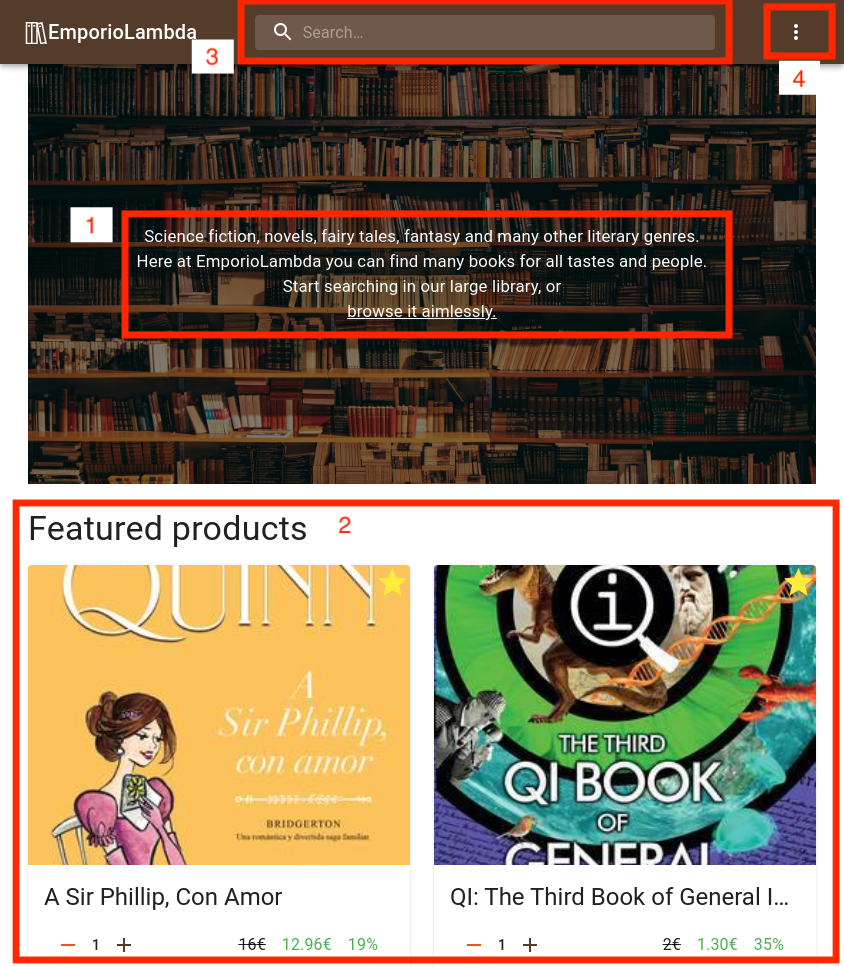
\includegraphics[scale=0.4]{Immagini/Acquirente/home_primo_accesso.png}
	\caption{Schermata principale}
	\label{fig:Home}
\end{figure}
Cliccando sull'icona del menù (4) appariranno due icone cliccabili dall'utente per poter visualizzare il proprio carrello o effettuare il login/registrazione.
\begin{figure}[H]
	\centering
	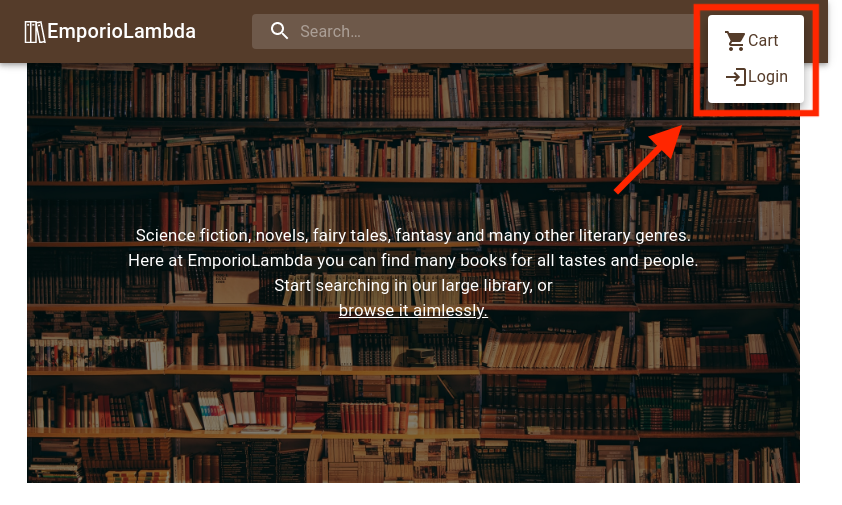
\includegraphics[scale=0.4]{Immagini/Acquirente/home-mobile-open.customer.png}
	\caption{Schermata principale con menù a tendina}
	\label{fig:Homeicone}
\end{figure}
\begin{figure}[h!]
	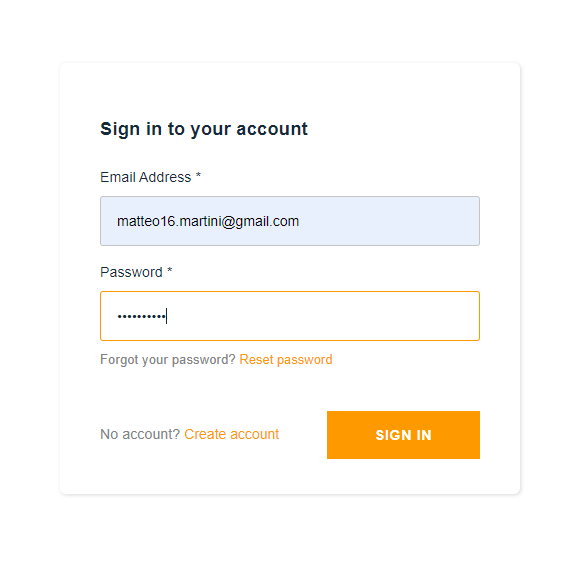
\includegraphics[scale=0.7]{Immagini/Acquirente/login.png}\quad
	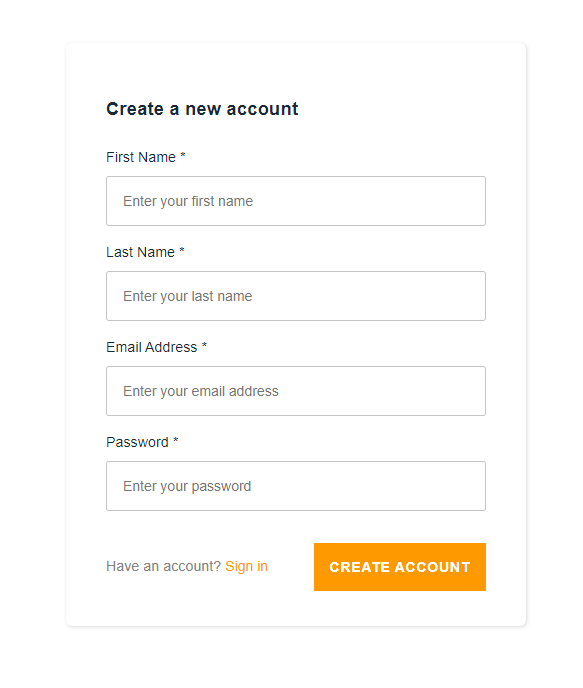
\includegraphics[scale=0.6]{Immagini/Acquirente/createAccount.png}
\end{figure}
\newpage
\section{Acquirente}\label{Acquirente}
La schermata principale visualizzata comprende nuovamente descrizione dell'azienda, prodotti in evidenza e:
\begin{enumerate}
	\item \glo{Icona} per accedere al carrello;
	\item Icona per effettuare il logout.
\end{enumerate} 
\begin{figure}[H]
	\centering
	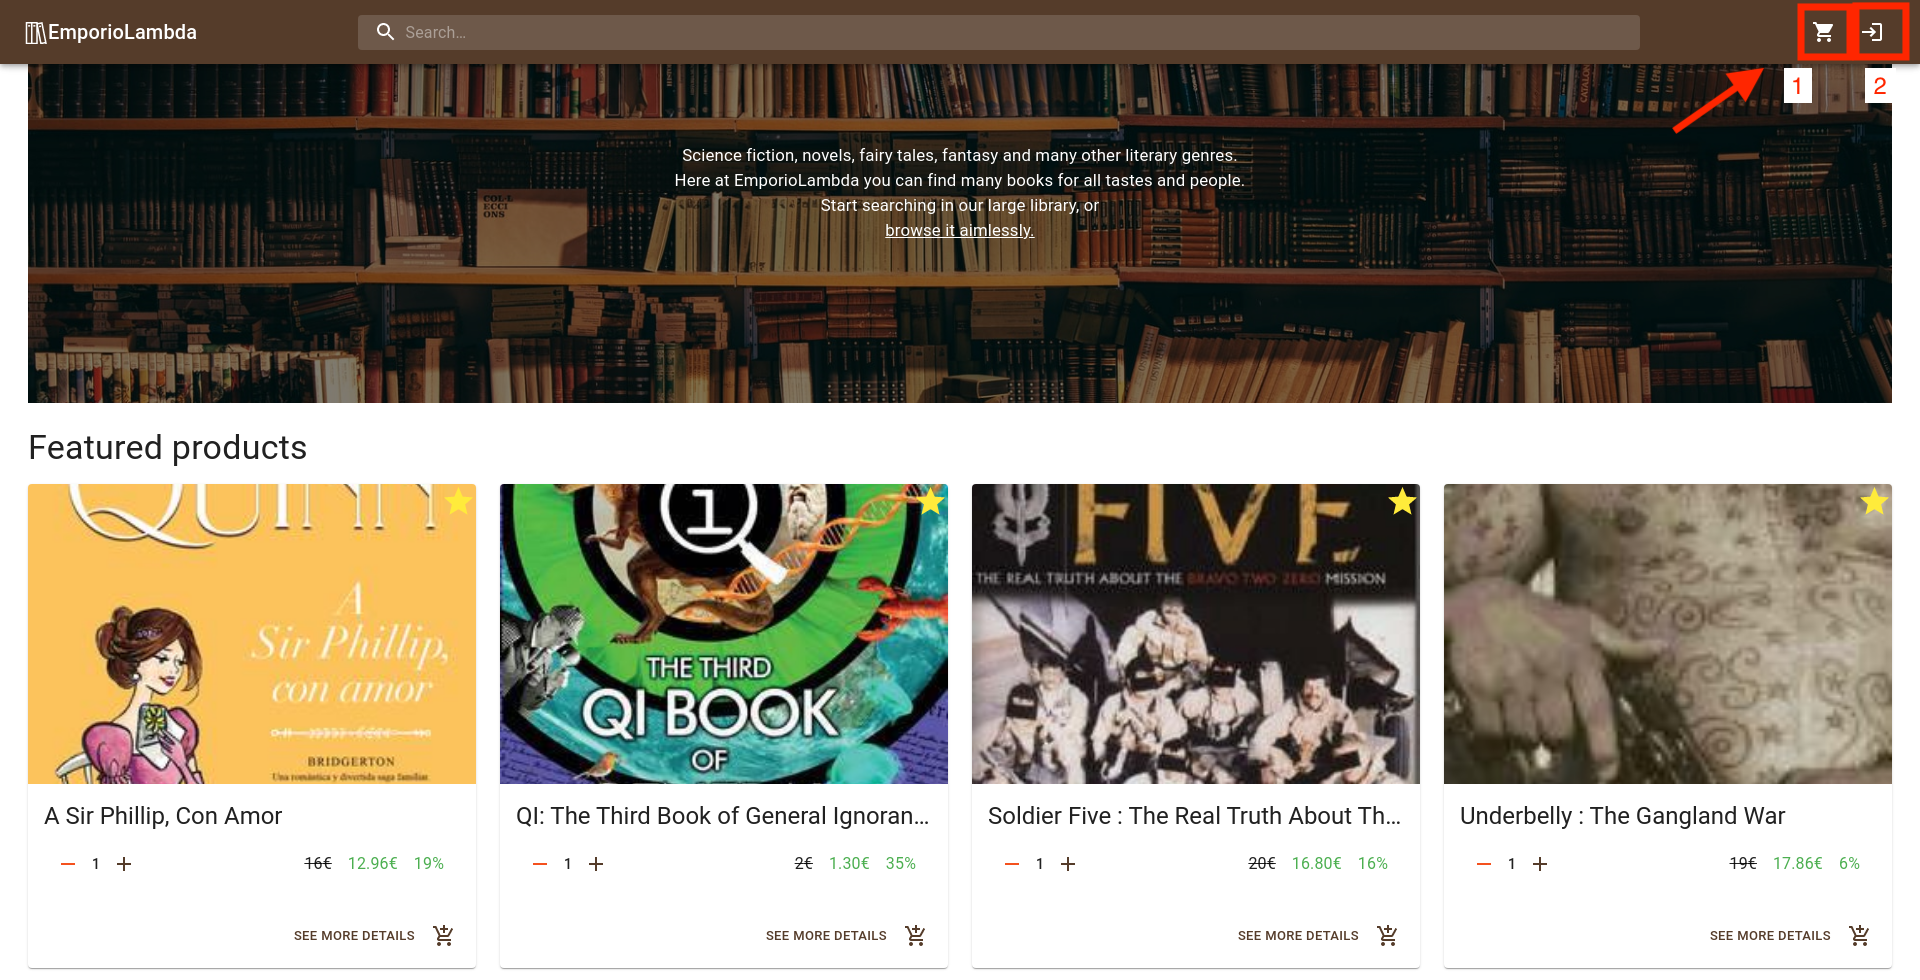
\includegraphics[scale=0.25]{Immagini/Acquirente/home.customer.png}
	\caption{Schermata principale utente autenticato}
	\label{fig:Homecustomer}
\end{figure}
\subsection{Visualizzazione specifiche di un prodotto}
L'acquirente, autenticato sulla piattaforma o come ospite, può visualizzare le specifiche di un prodotto in evidenza cliccando sullo stesso. La schermata alla quale sarà indirizzato comprenderà:
\begin{enumerate}
	\item Nome del prodotto;
	\item Elenco di immagini visualizzabili;
	\item Descrizione del prodotto;
	\item Prezzo ed eventuali sconti percentuali applicati;
	\item Categorie di appartenenza;
	\item Icone per modificare la quantità da inserire nel carrello e per inserire i prodotti nel carrello.
\end{enumerate} 
\begin{figure}[H]
	\centering
	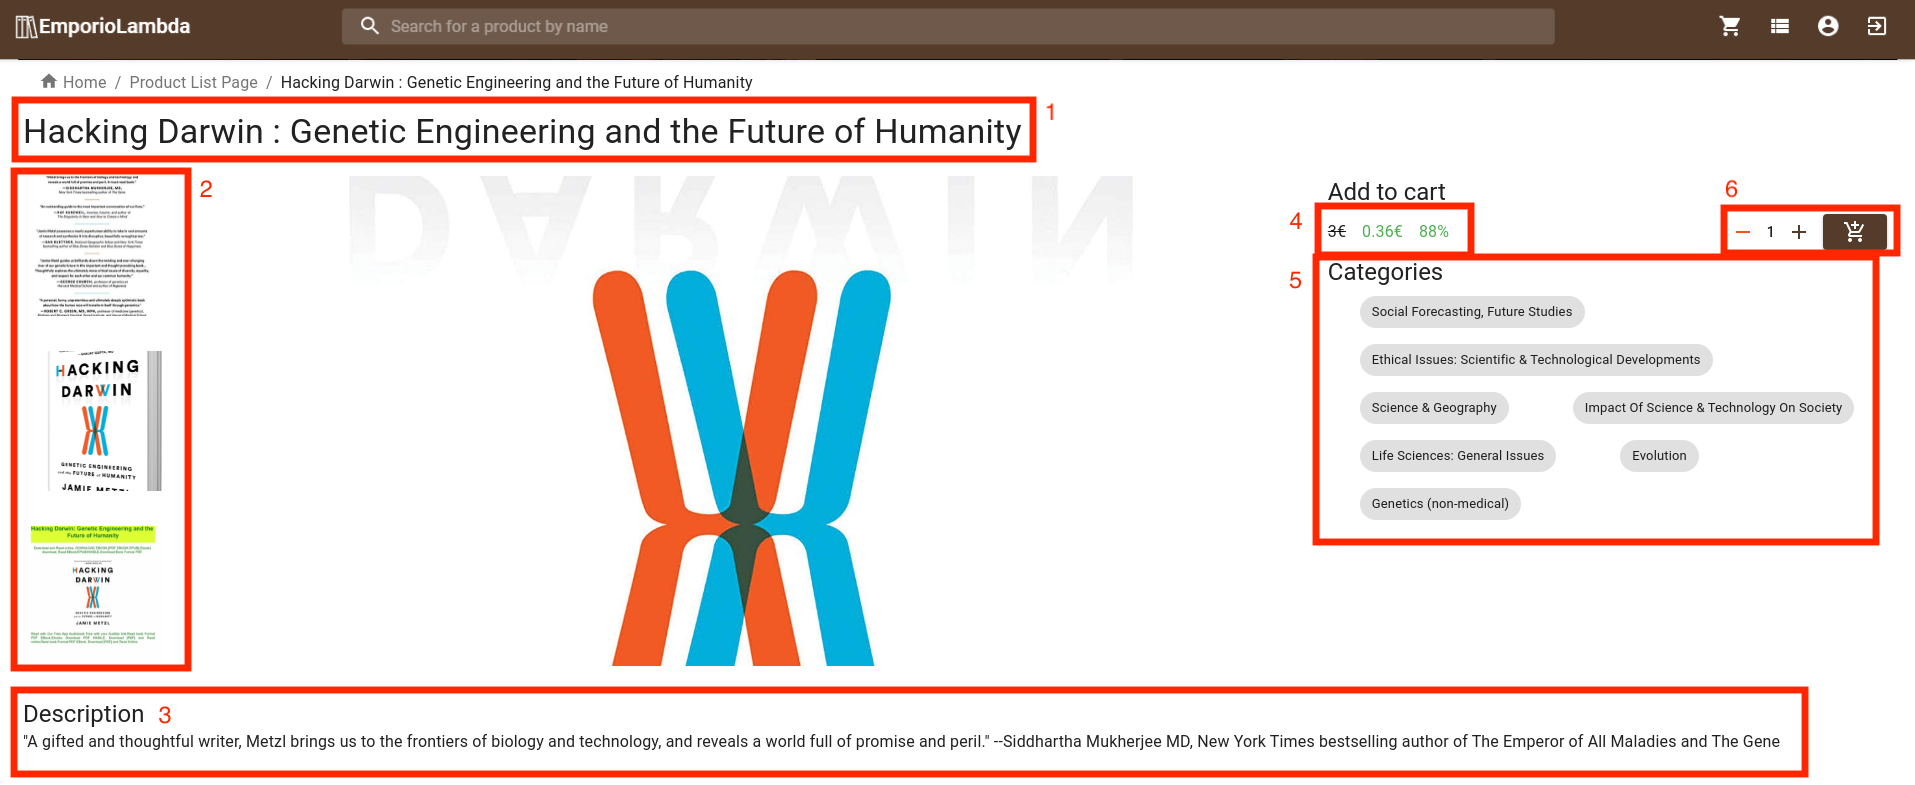
\includegraphics[scale=0.25]{Immagini/Acquirente/pdp.customer.png}
	\caption{Specifiche di un prodotto}
	\label{fig:SpecificheProdotto}
\end{figure}
\subsection{Visualizzazione elenco prodotti}
L'utente può visualizzare l'intero elenco di prodotti presenti nella piattaforma, per ognuno di essi sarà visualizzato nome, prezzo ed eventuali sconti, icone per modificare il numero di prodotti da inserire nel carrello e per inserire la quantità nel carrello. I prodotti non disponibili avranno un'indicazione sopra l'immagine del prodotto.
\begin{figure}[H]
	\centering
	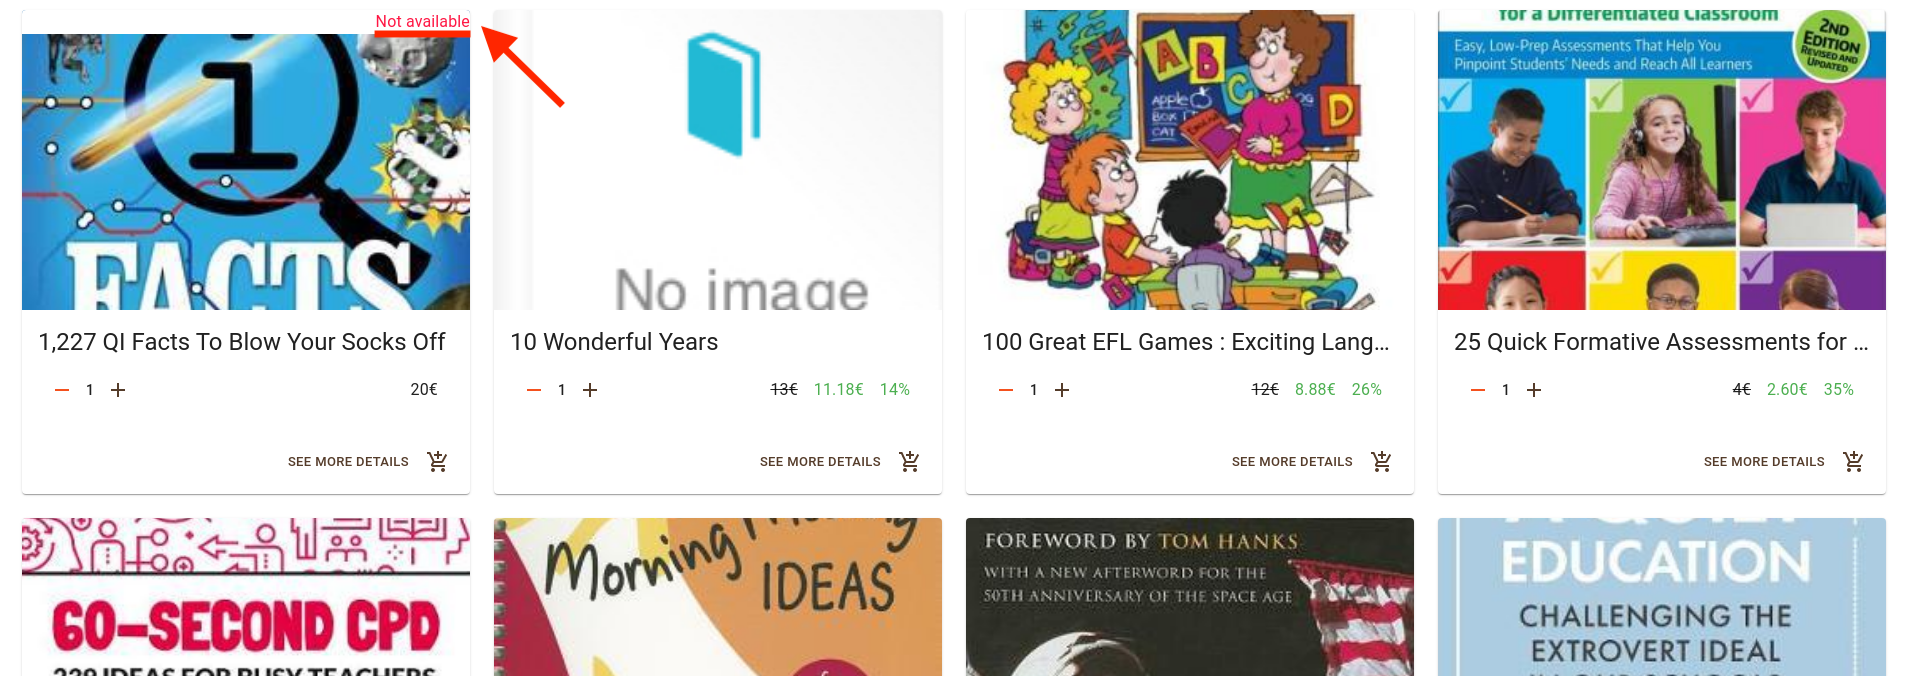
\includegraphics[scale=0.25]{Immagini/Acquirente/plp-pagination.customer.png}
	\caption{Schermata dei prodotti nella piattaforma}
	\label{fig:PLP}
\end{figure}
I prodotti possono essere visualizzati secondo un preciso ordine cliccando sull'apposita icona e selezionando il tipo di ordinamento desiderato.
\begin{figure}[H]
	\centering
	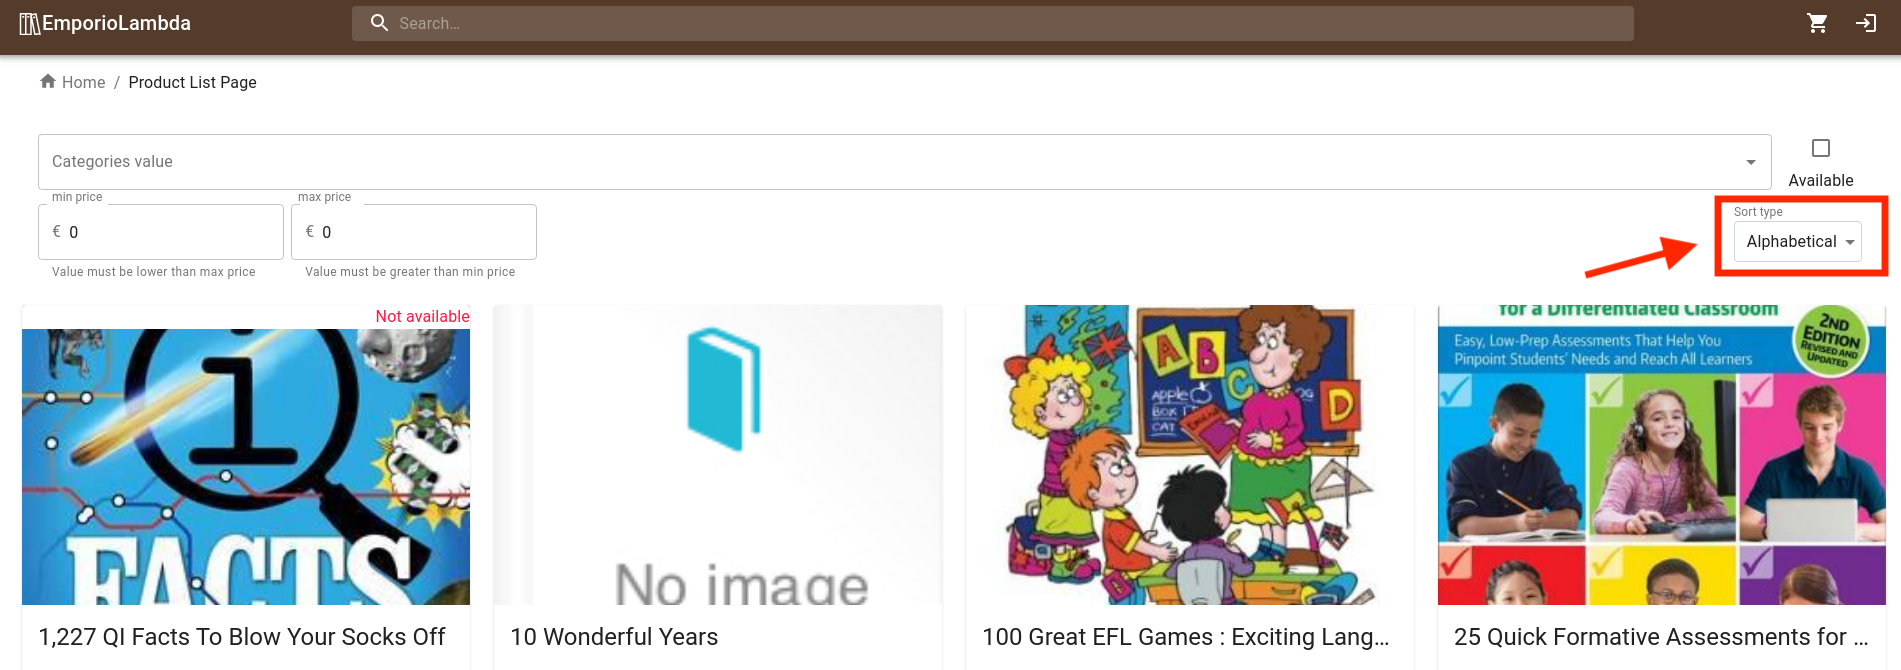
\includegraphics[scale=0.25]{Immagini/Acquirente/plp-sort1.png}
	\caption{Schermata dei prodotti nella piattaforma con ordinamento}
	\label{fig:PLPordinamento1}
\end{figure}
\begin{figure}[H]
	\centering
	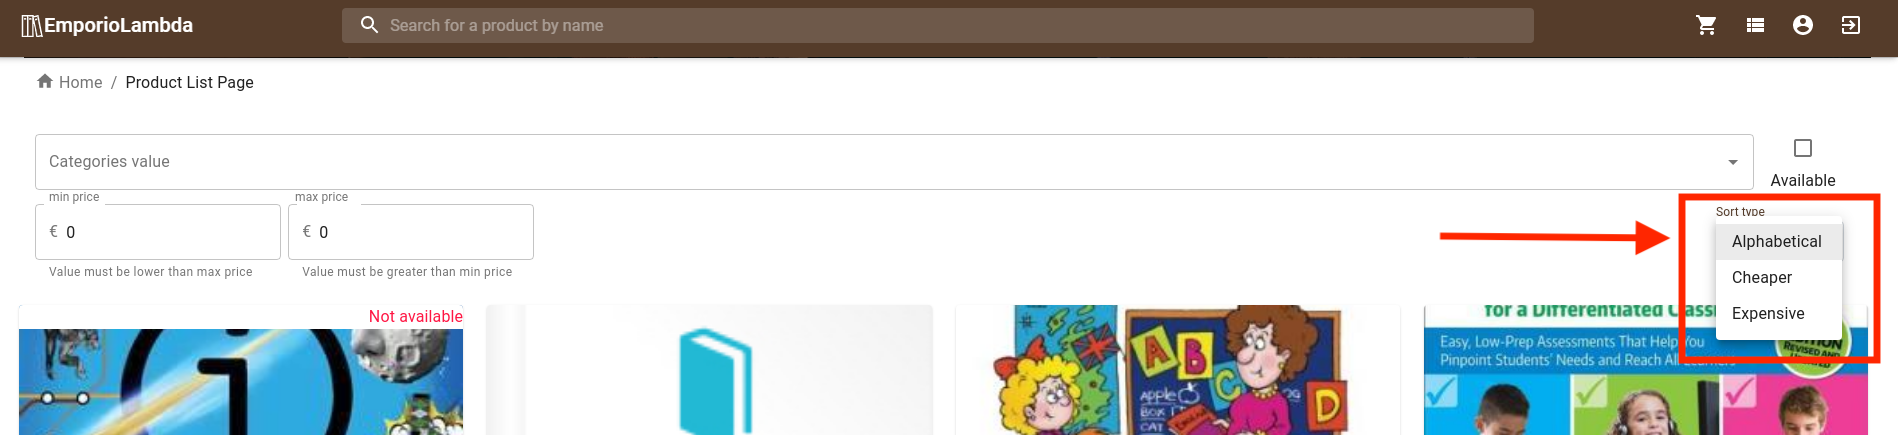
\includegraphics[scale=0.25]{Immagini/Acquirente/plp-sort-filter.png}
	\caption{Schermata dei prodotti nella piattaforma con possibili ordinamenti}
	\label{fig:PLPordinamento2}
\end{figure}
\subsection{Filtraggio dei prodotti}
Nella schermata con l'elenco prodotti l'utente può procedere a raffinare la sua ricerca impostando una serie di filtri.
\begin{figure}[H]
	\centering
	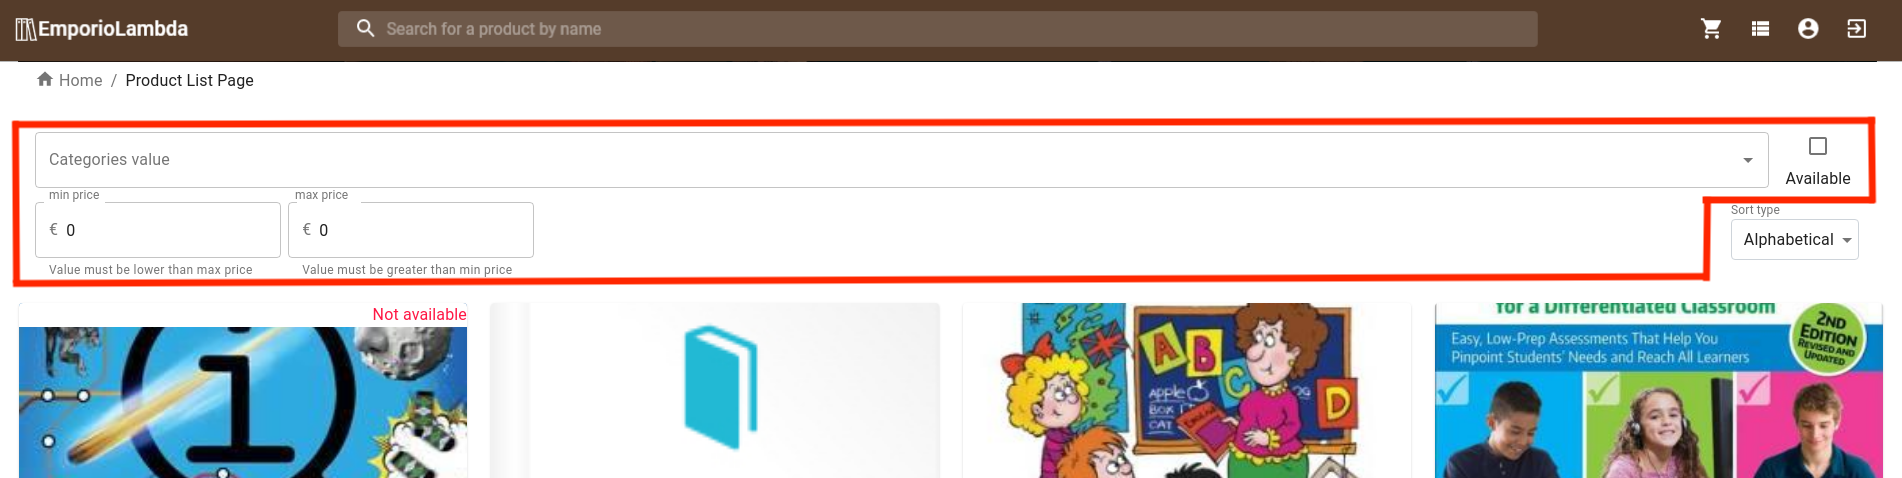
\includegraphics[scale=0.25]{Immagini/Acquirente/plp-filter.customer.png}
	\caption{Schermata dei prodotti con filtri applicabili}
	\label{fig:PLPfiltri}
\end{figure}
\subsubsection{Filtro prodotti per categorie}
Per ricercare un prodotto in base alle categorie di appartenenza, l'utente può cliccare sulla prima barra di ricerca e selezionare le categorie di interesse tra quelle visualizzate.
\begin{figure}[H]
	\centering
	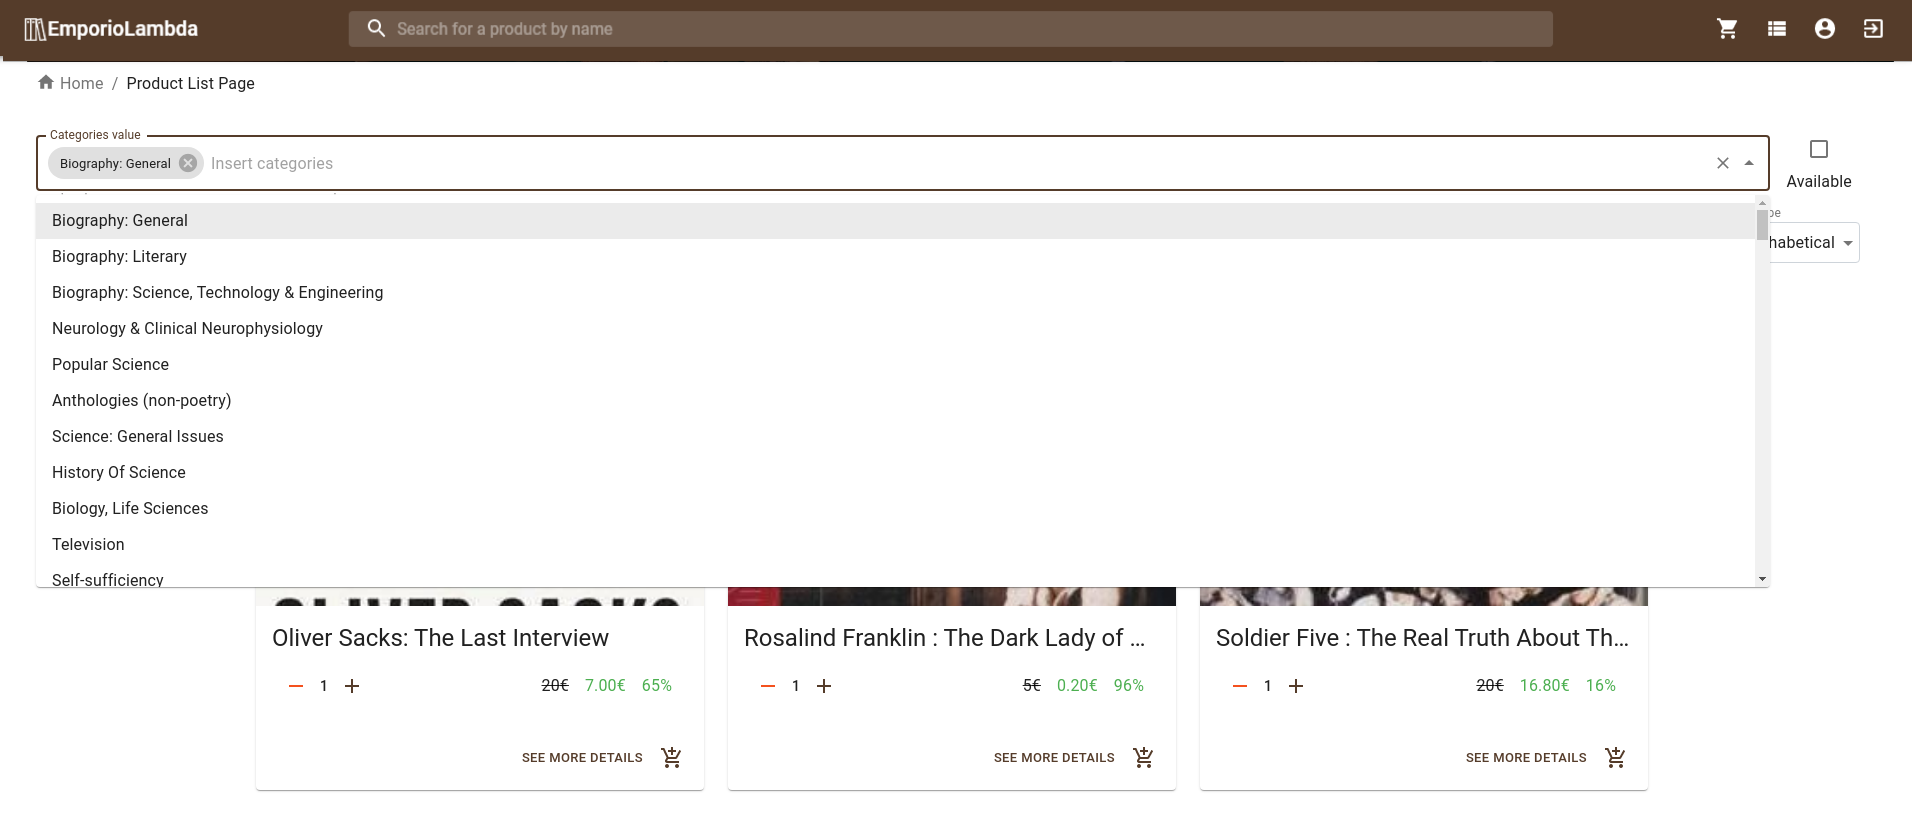
\includegraphics[scale=0.25]{Immagini/Acquirente/plp-categories-open.png}
	\caption{Filtro prodotti per categorie}
	\label{fig:PLPcategorie}
\end{figure}
\subsubsection{Filtro prodotti per disponibilità}
Per visualizzare i prodotti in base alla loro disponibilità, l'utente può selezionare la casella indicata.
\begin{figure}[H]
	\centering
	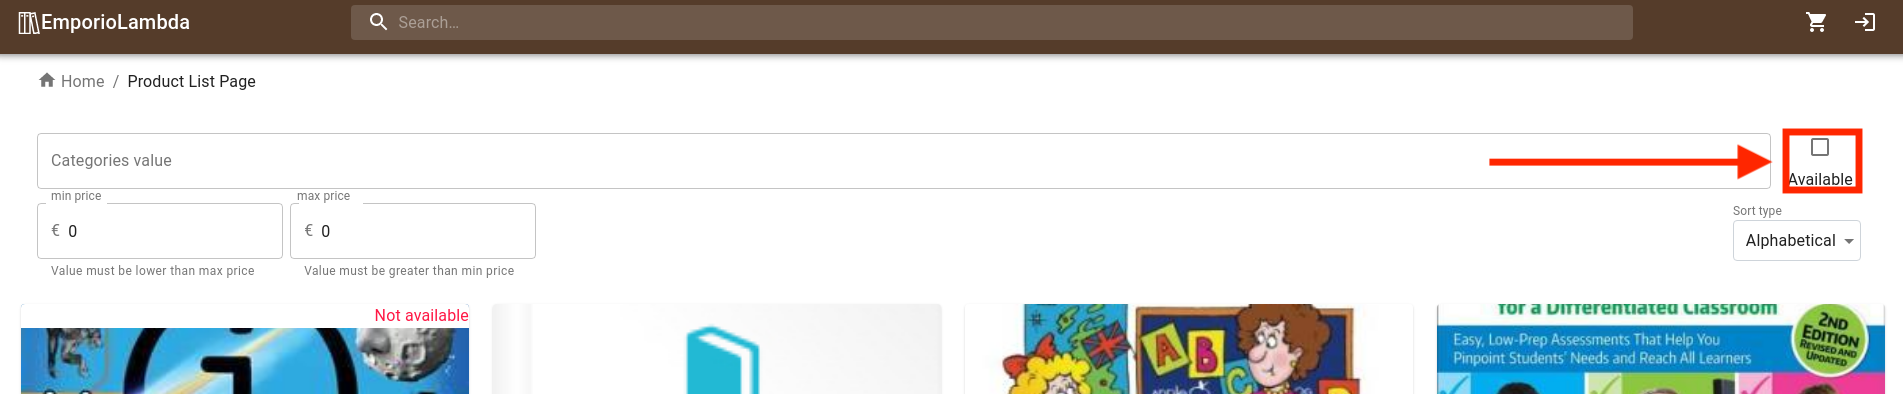
\includegraphics[scale=0.25]{Immagini/Acquirente/plp-available.png}
	\caption{Filtro prodotti per disponibilità}
	\label{fig:PLPdisponibilità}
\end{figure}
\subsubsection{Filtro prodotti per prezzo}
Per visualizzare i prodotti in base al loro prezzo, l'utente può inserire nelle caselle (1) e (2) il valore minimo e massimo per effettuare la ricerca.
\begin{figure}[H]
	\centering
	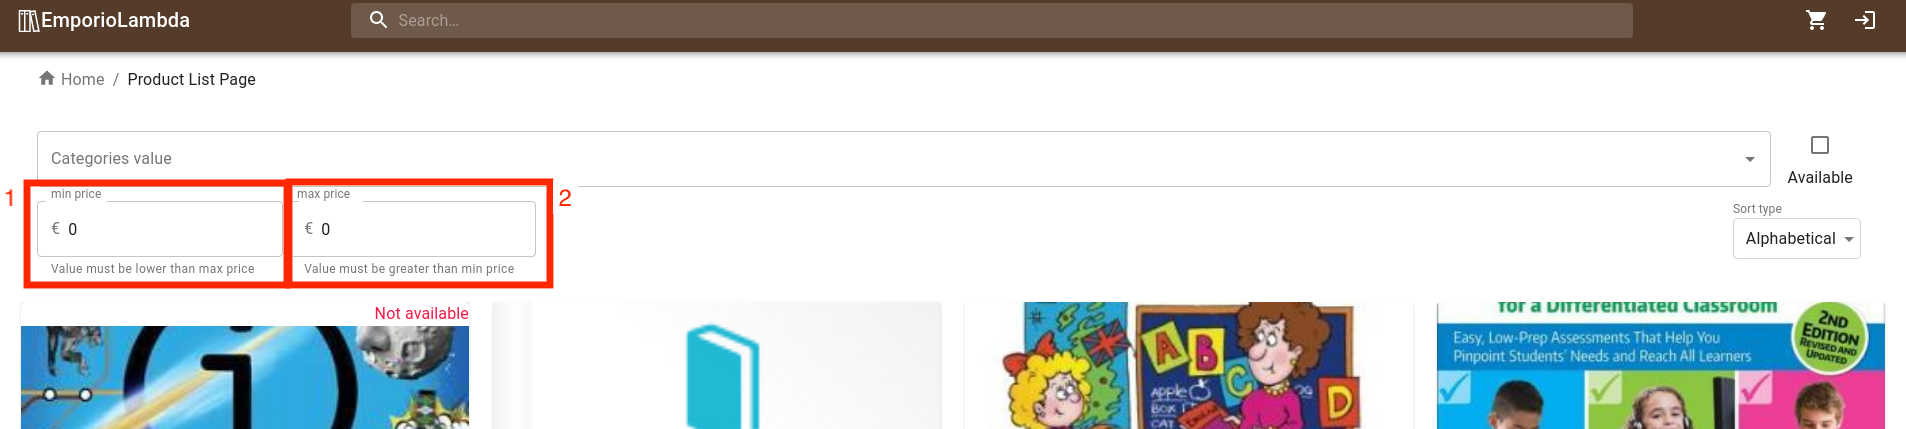
\includegraphics[scale=0.25]{Immagini/Acquirente/plp-price.png}
	\caption{Filtro prodotti per prezzo}
	\label{fig:PLPprezzo}
\end{figure}
\subsection{Visualizzazione del carrello}
Premendo sull'icona del carrello presente in ogni schermata è possibile per l'utente accedere al proprio carrello. Verranno visualizzati oltre ai vari prodotti con le loro informazioni:
\begin{enumerate}
	\item Prezzo totale;
	\item Icona per procedere al pagamento.
\end{enumerate} 
\begin{figure}[H]
	\centering
	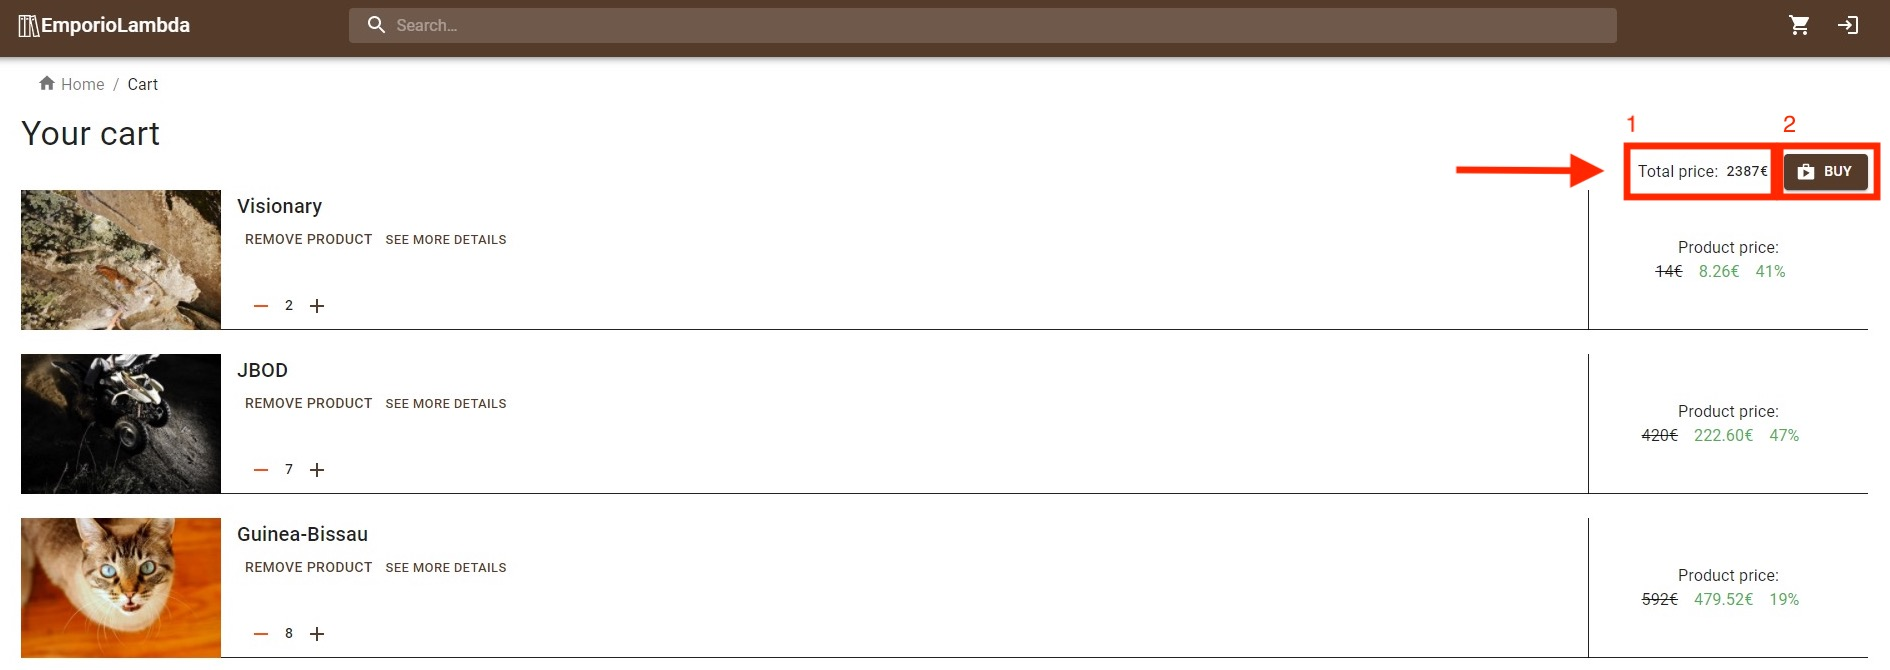
\includegraphics[scale=0.25]{Immagini/Acquirente/Cart.JPG}
	\caption{Carrello}
	\label{fig:Carrello}
\end{figure}
\subsection{Pagamento e gestione della spedizione}
Dopo aver cliccato sull'icona per procedere al pagamento si verrà reindirizzati ad una schermata di riepilogo prima di procedere con l'effettivo checkout.
Nella schermata è possibile visualizzare nuovamente l'elenco dei vari prodotti presenti nel carrello cliccando sull'apposita icona.
\begin{figure}[H]
	\centering
	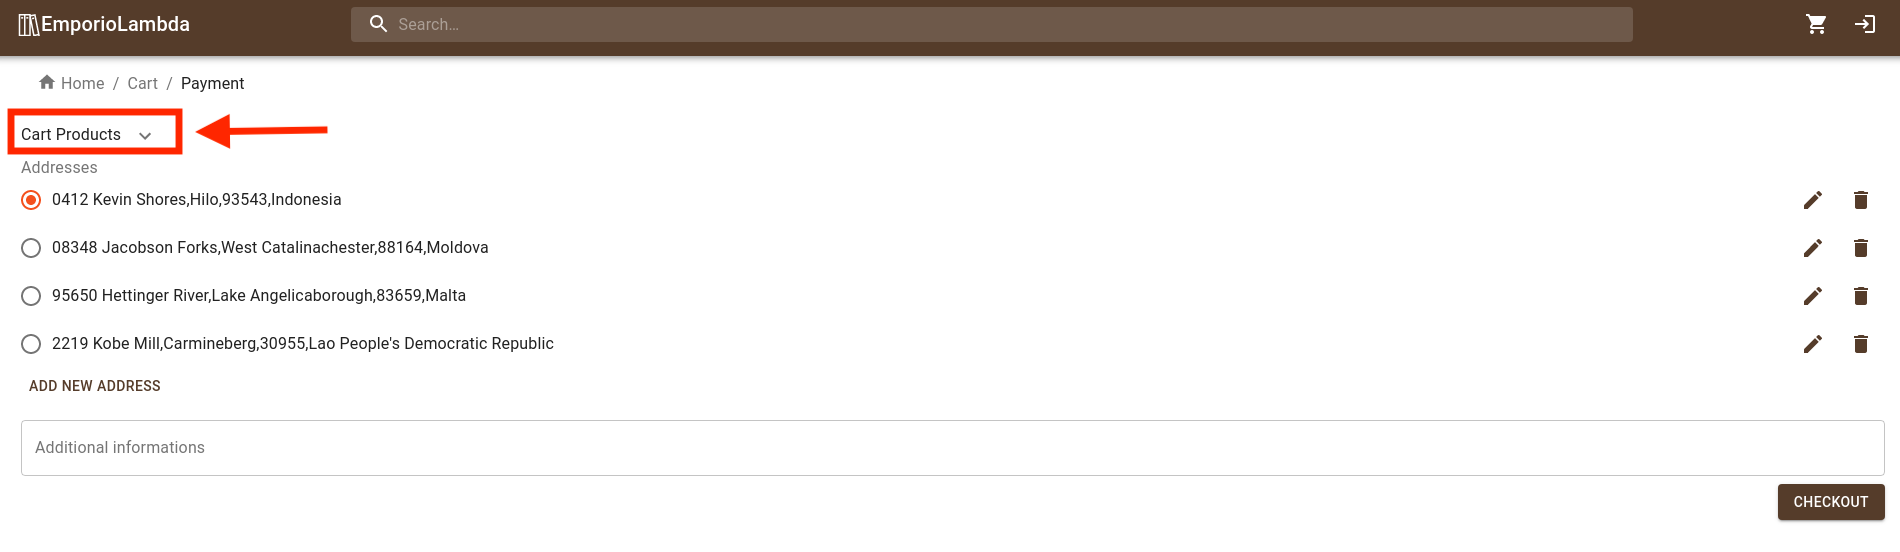
\includegraphics[scale=0.25]{Immagini/Acquirente/payment.cartproduct.png}
	\caption{Schermata di riepilogo prima del checkout}
	\label{fig:CartProduct}
\end{figure}
\begin{figure}[H]
	\centering
	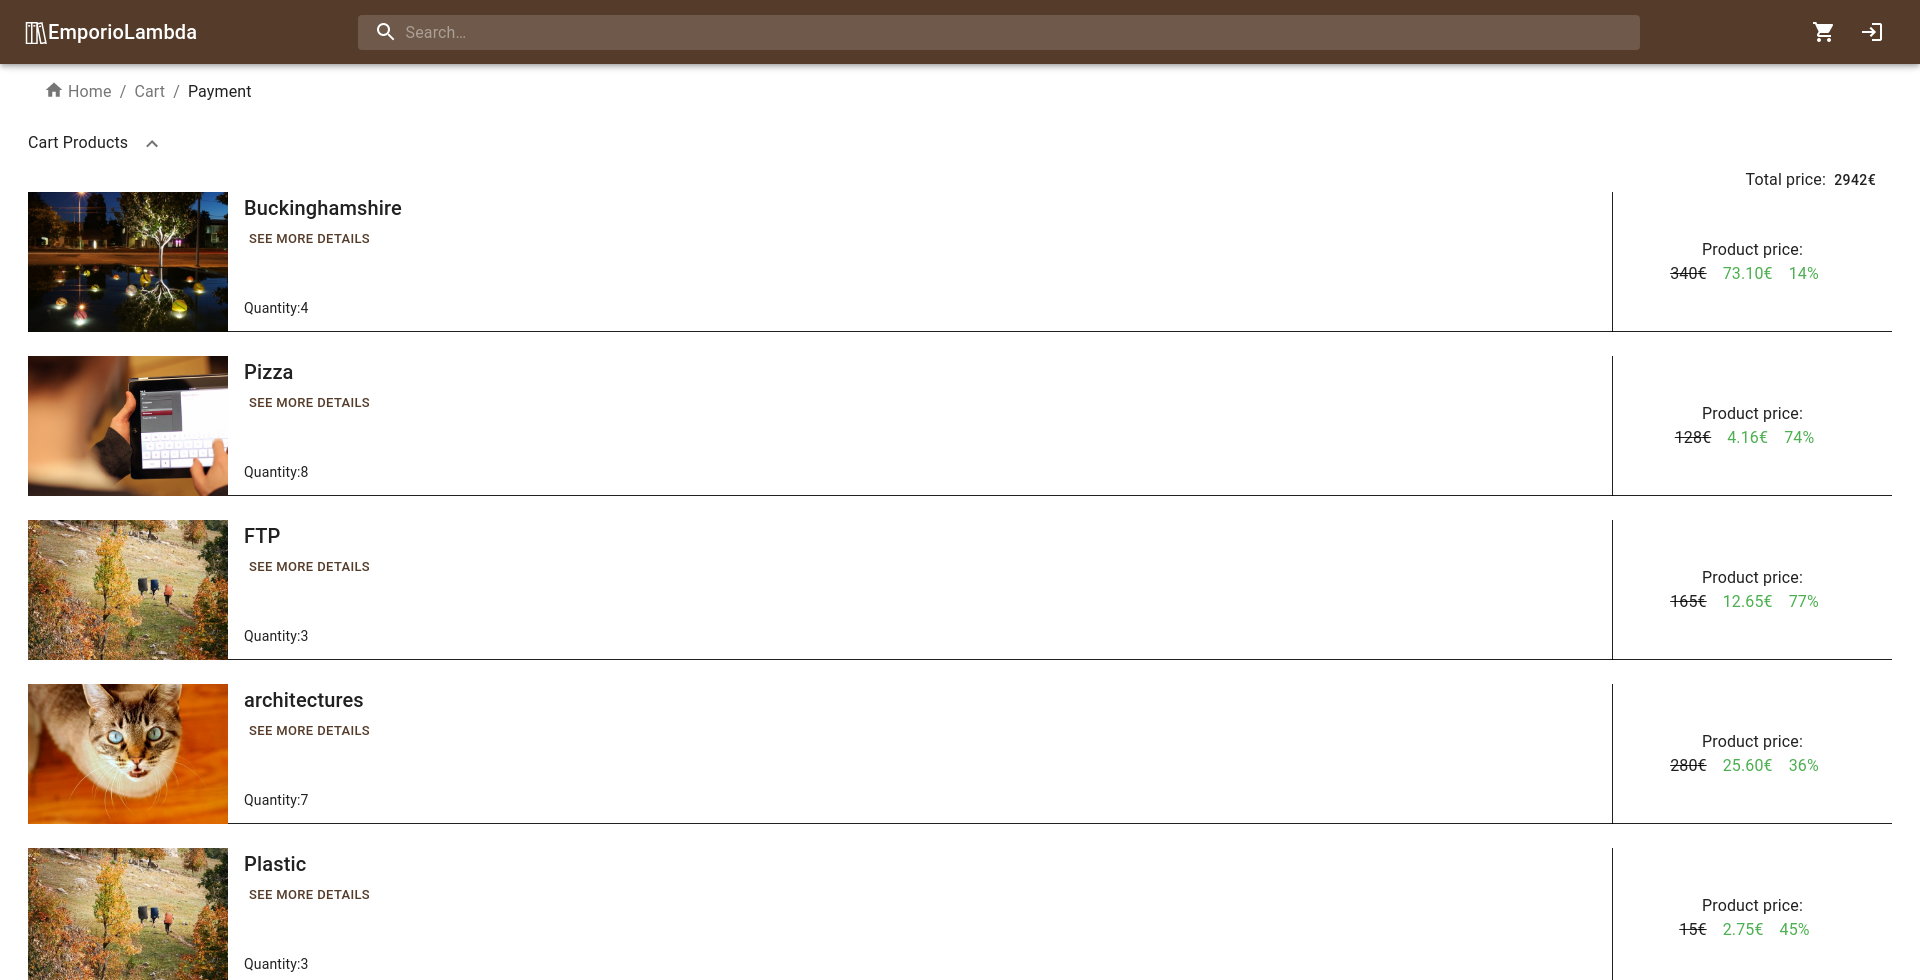
\includegraphics[scale=0.25]{Immagini/Acquirente/payment-products-open.customer.png}
	\caption{Schermata elenco prodotti nel carrello}
	\label{fig:CartProductElenco}
\end{figure}
Potranno essere inserite delle informazioni aggiuntive per il venditore.
\begin{figure}[H]
	\centering
	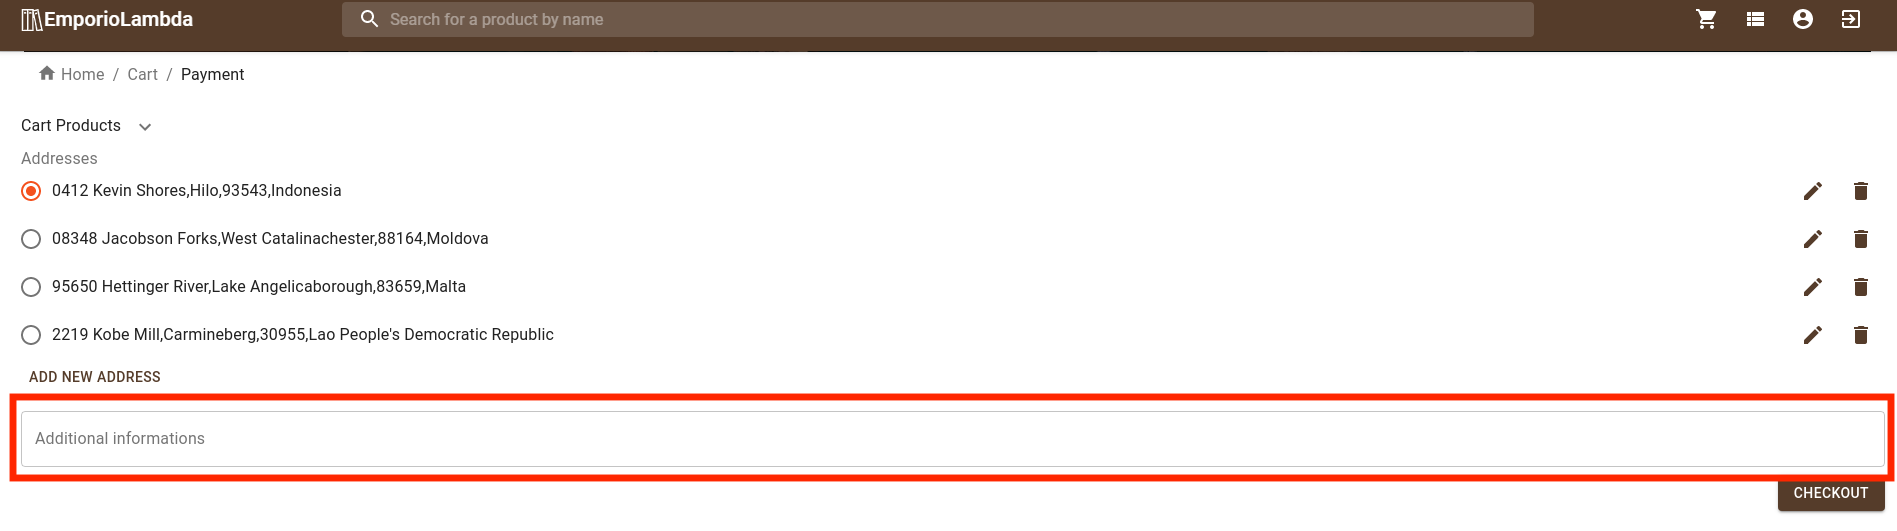
\includegraphics[scale=0.25]{Immagini/Acquirente/payment.addinfo.png}
	\caption{Schermata elenco di riepilogo prima del checkout con \glo{form} per inserimento informazioni aggiuntive}
	\label{fig:CartAddinfo}
\end{figure}
Nella stessa schermata sarà possibile gestire gli indirizzi di spedizione precedentemente inseriti, inserirne uno nuovo e selezionare l'indirizzo prescelto per l'ordine.
\begin{figure}[H]
	\centering
	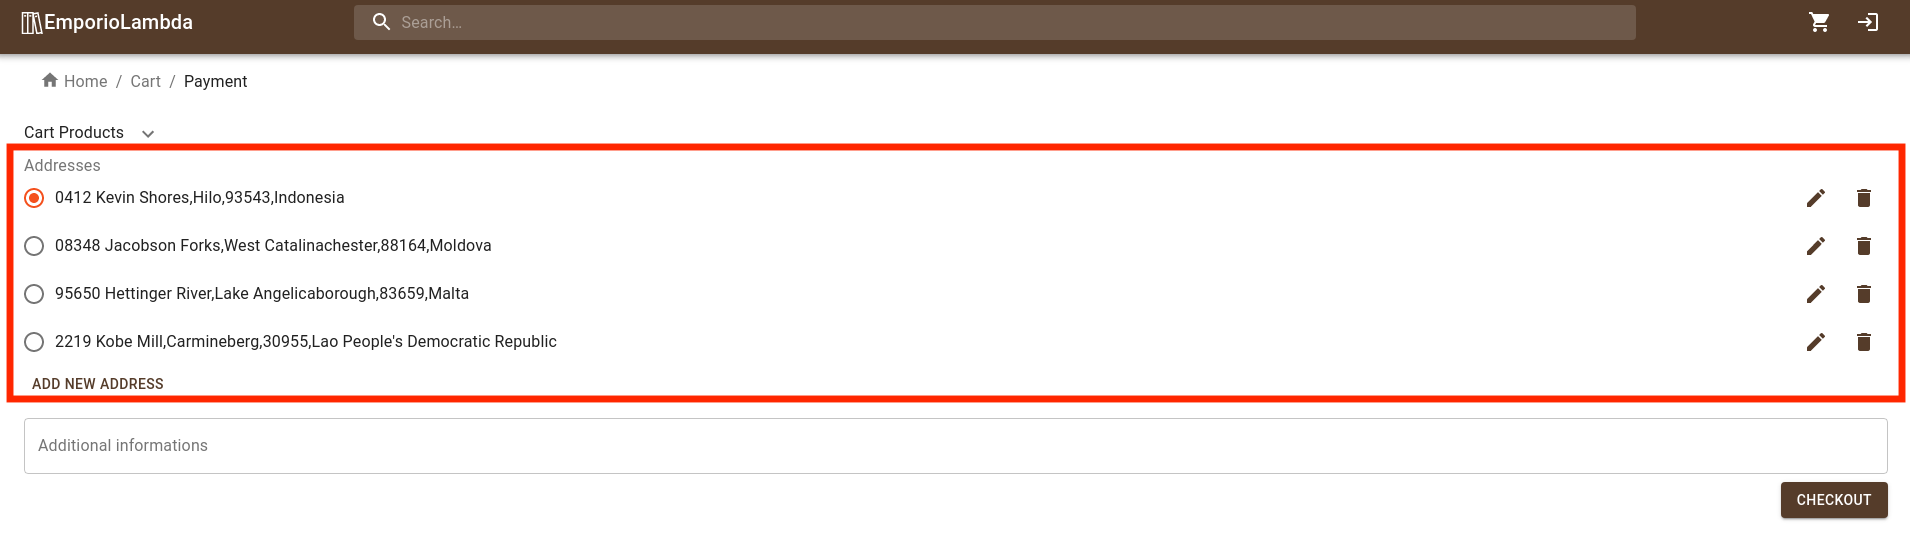
\includegraphics[scale=0.25]{Immagini/Acquirente/payment.customer.png}
	\caption{Schermata di riepilogo prima del checkout in cui gestire gli indirizzi}
	\label{fig:CartAddress}
\end{figure}
\subsubsection{Inserimento nuovo indirizzo}
Per inserire un nuovo indirizzo l'utente deve premere sulla scritta apposita, apparirà un \glo{form} in cui potrà inserire i vari dati relativi al nuovo indirizzo.
\begin{figure}[H]
	\centering
	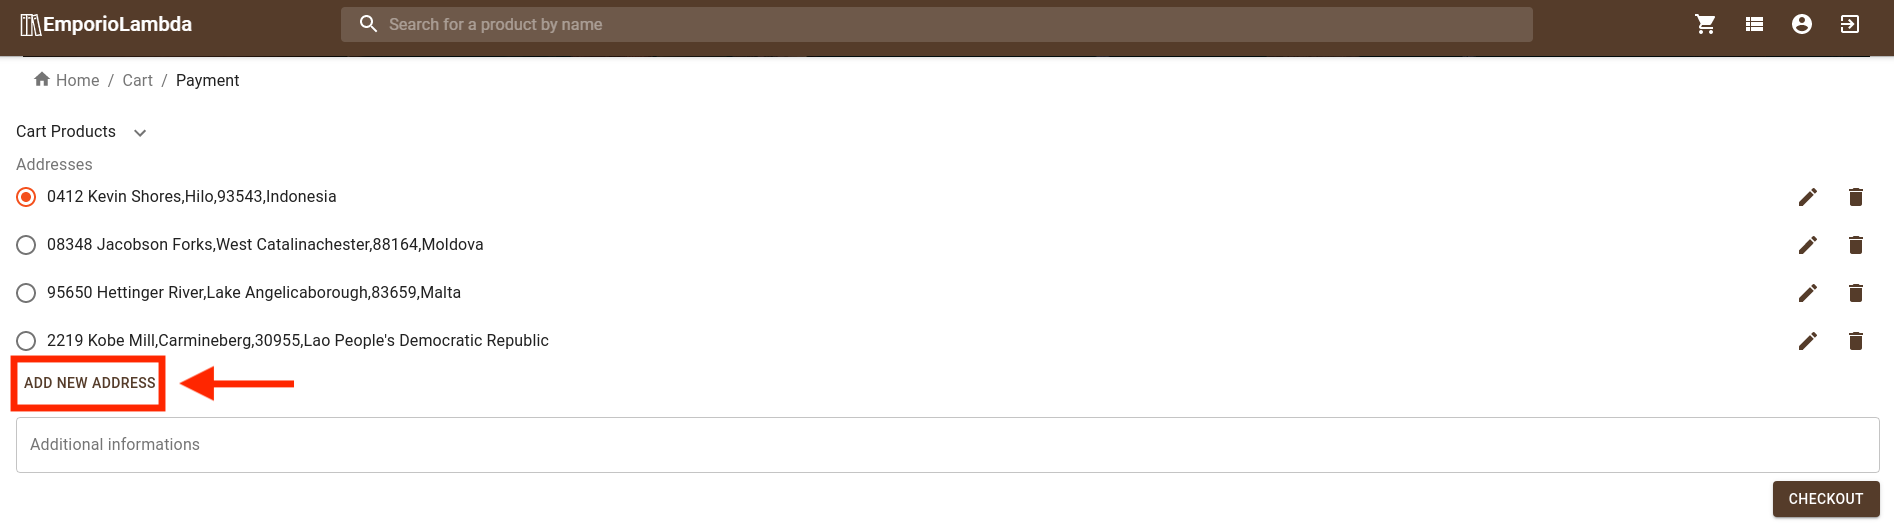
\includegraphics[scale=0.25]{Immagini/Acquirente/payment.addressnew.png}
	\caption{Schermata di riepilogo prima del checkout per inserire nuovo indirizzo}
	\label{fig:NewAddress}
\end{figure}
\begin{figure}[H]
	\centering
	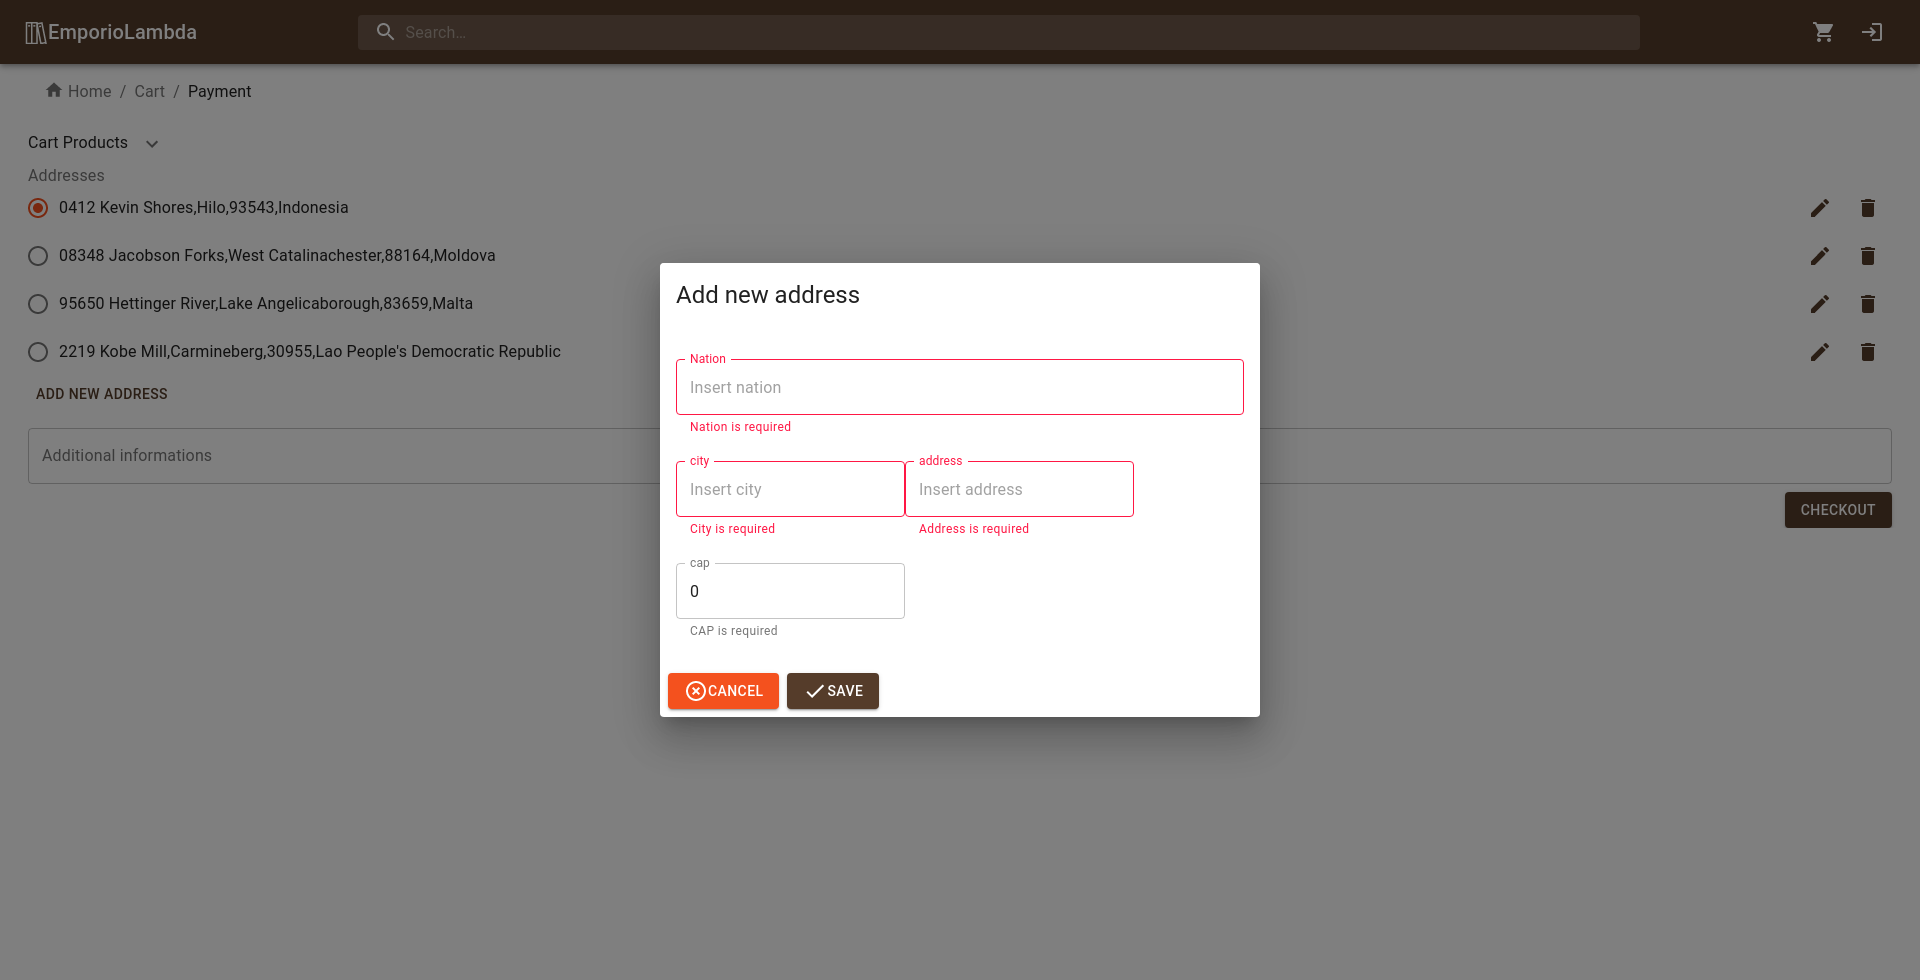
\includegraphics[scale=0.25]{Immagini/Acquirente/payment-new-address.customer.png}
	\caption{Form di inserimento nuovo indirizzo}
	\label{fig:CartnewAddress}
\end{figure}
\subsubsection{Eliminazione di un indirizzo inserito precedentemente}
Per eliminare un indirizzo precedentemente inserito l'utente deve cliccare sull'icona del cestino e confermare l'eliminazione.
\begin{figure}[H]
	\centering
	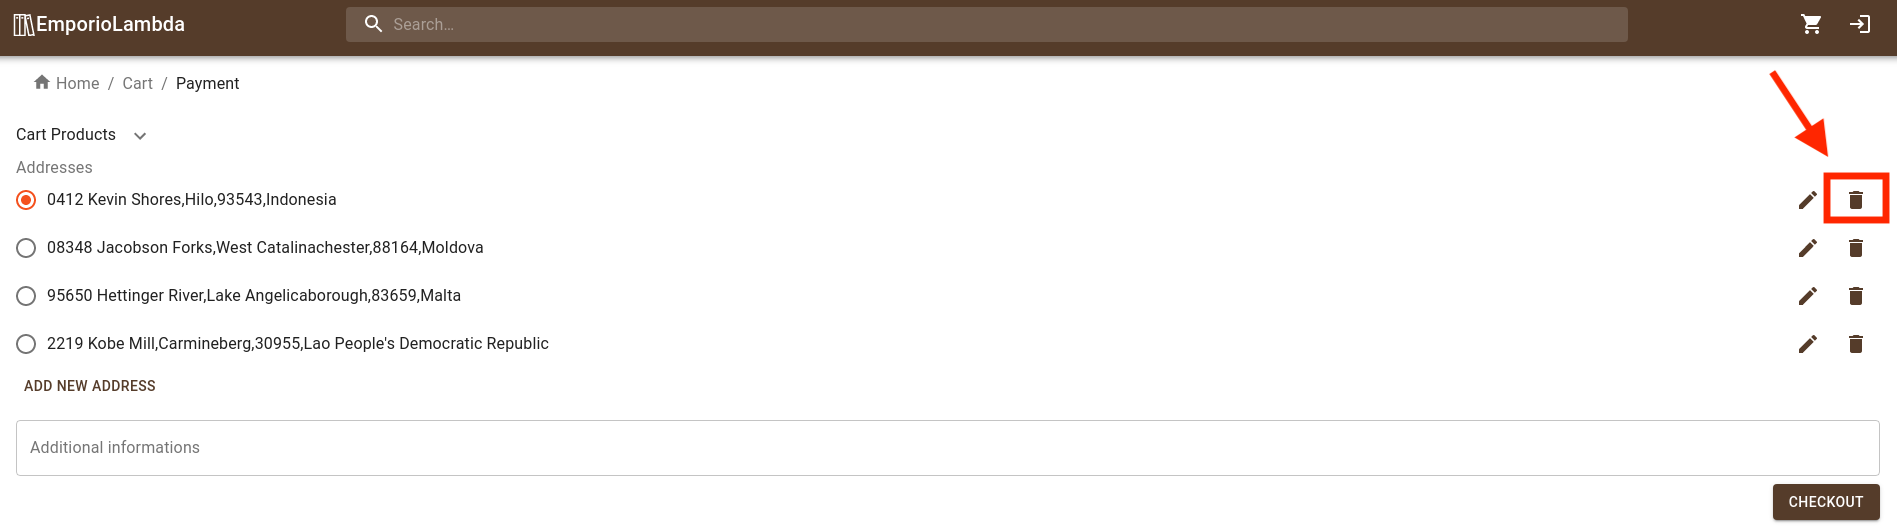
\includegraphics[scale=0.25]{Immagini/Acquirente/payment.addressdelete.png}
	\caption{Schermata di riepilogo prima del checkout per eliminare un indirizzo}
	\label{fig:DeleteAddress}
\end{figure}
\begin{figure}[H]
	\centering
	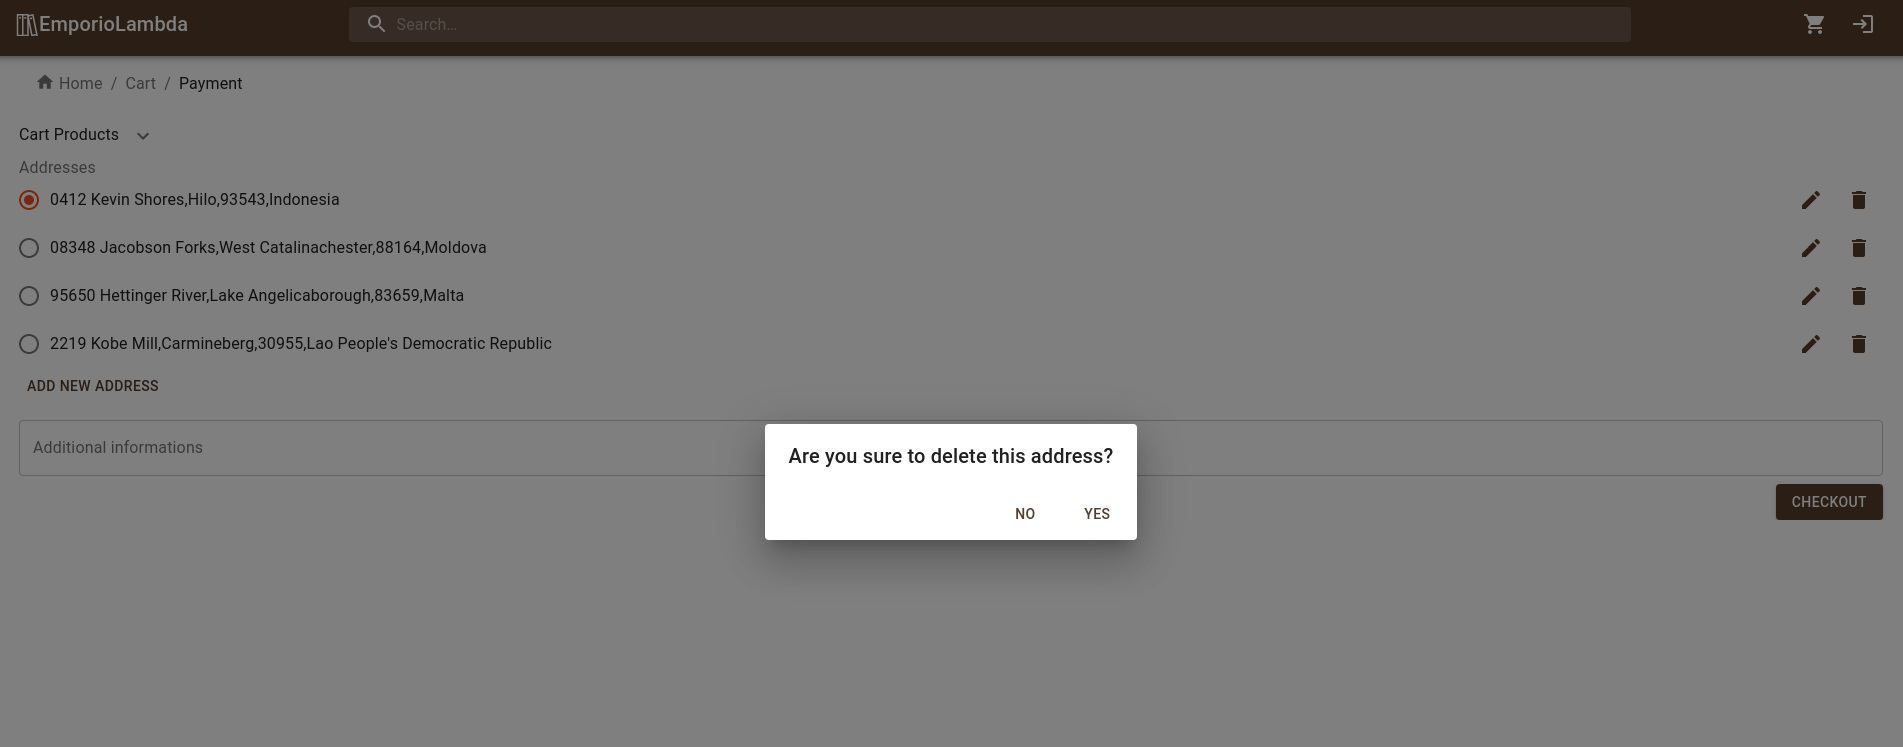
\includegraphics[scale=0.25]{Immagini/Acquirente/payment-delete-address.customer.png}
	\caption{Form di conferma eliminazione indirizzo}
	\label{fig:CartDeleteAddress}
\end{figure}
\subsubsection{Modifica di indirizzo inserito precedentemente}
Per modificare un indirizzo precedentemente inserito l'utente deve cliccare sull'icona della penna, si aprirà il form per modificare l'indirizzo.
\begin{figure}[H]
	\centering
	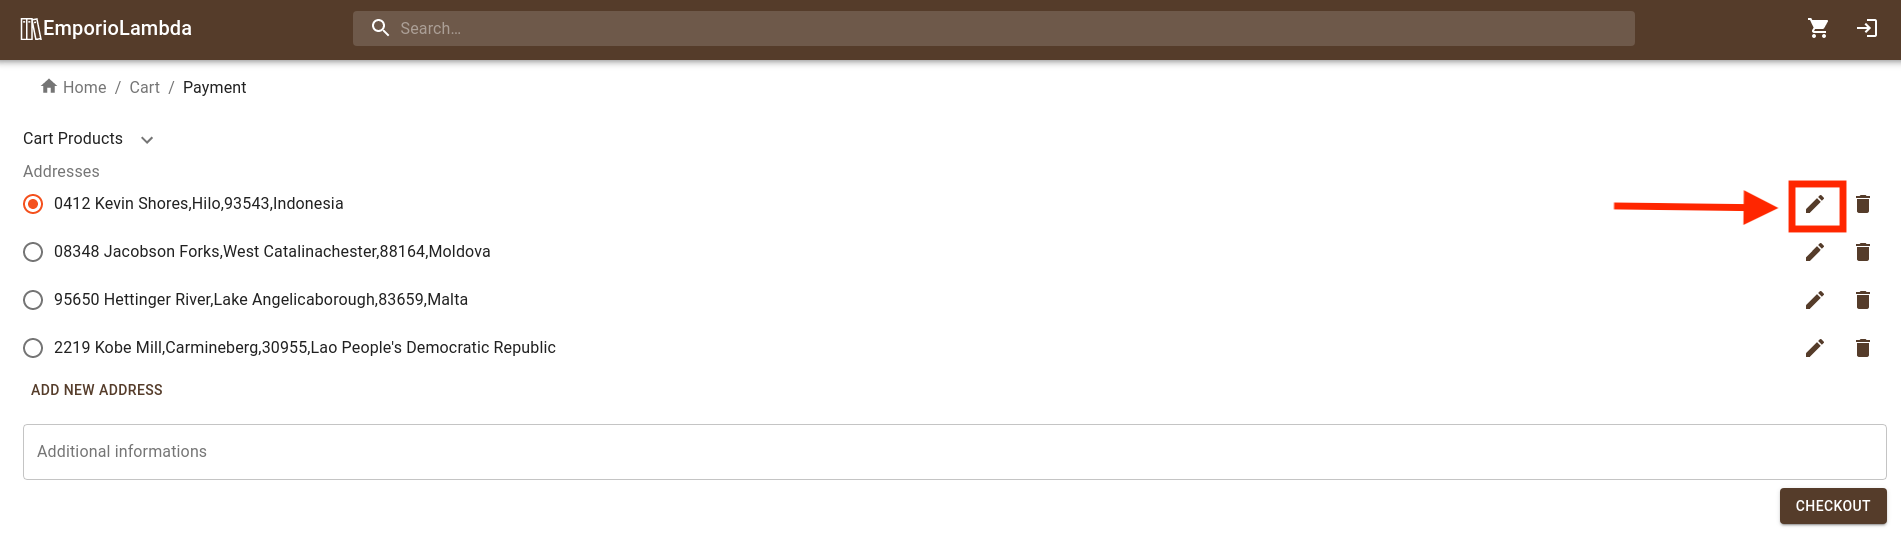
\includegraphics[scale=0.25]{Immagini/Acquirente/payment.addressmodify.png}
	\caption{Schermata di riepilogo prima del checkout per modificare un indirizzo}
	\label{fig:EditAddress}
\end{figure}
\begin{figure}[H]
	\centering
	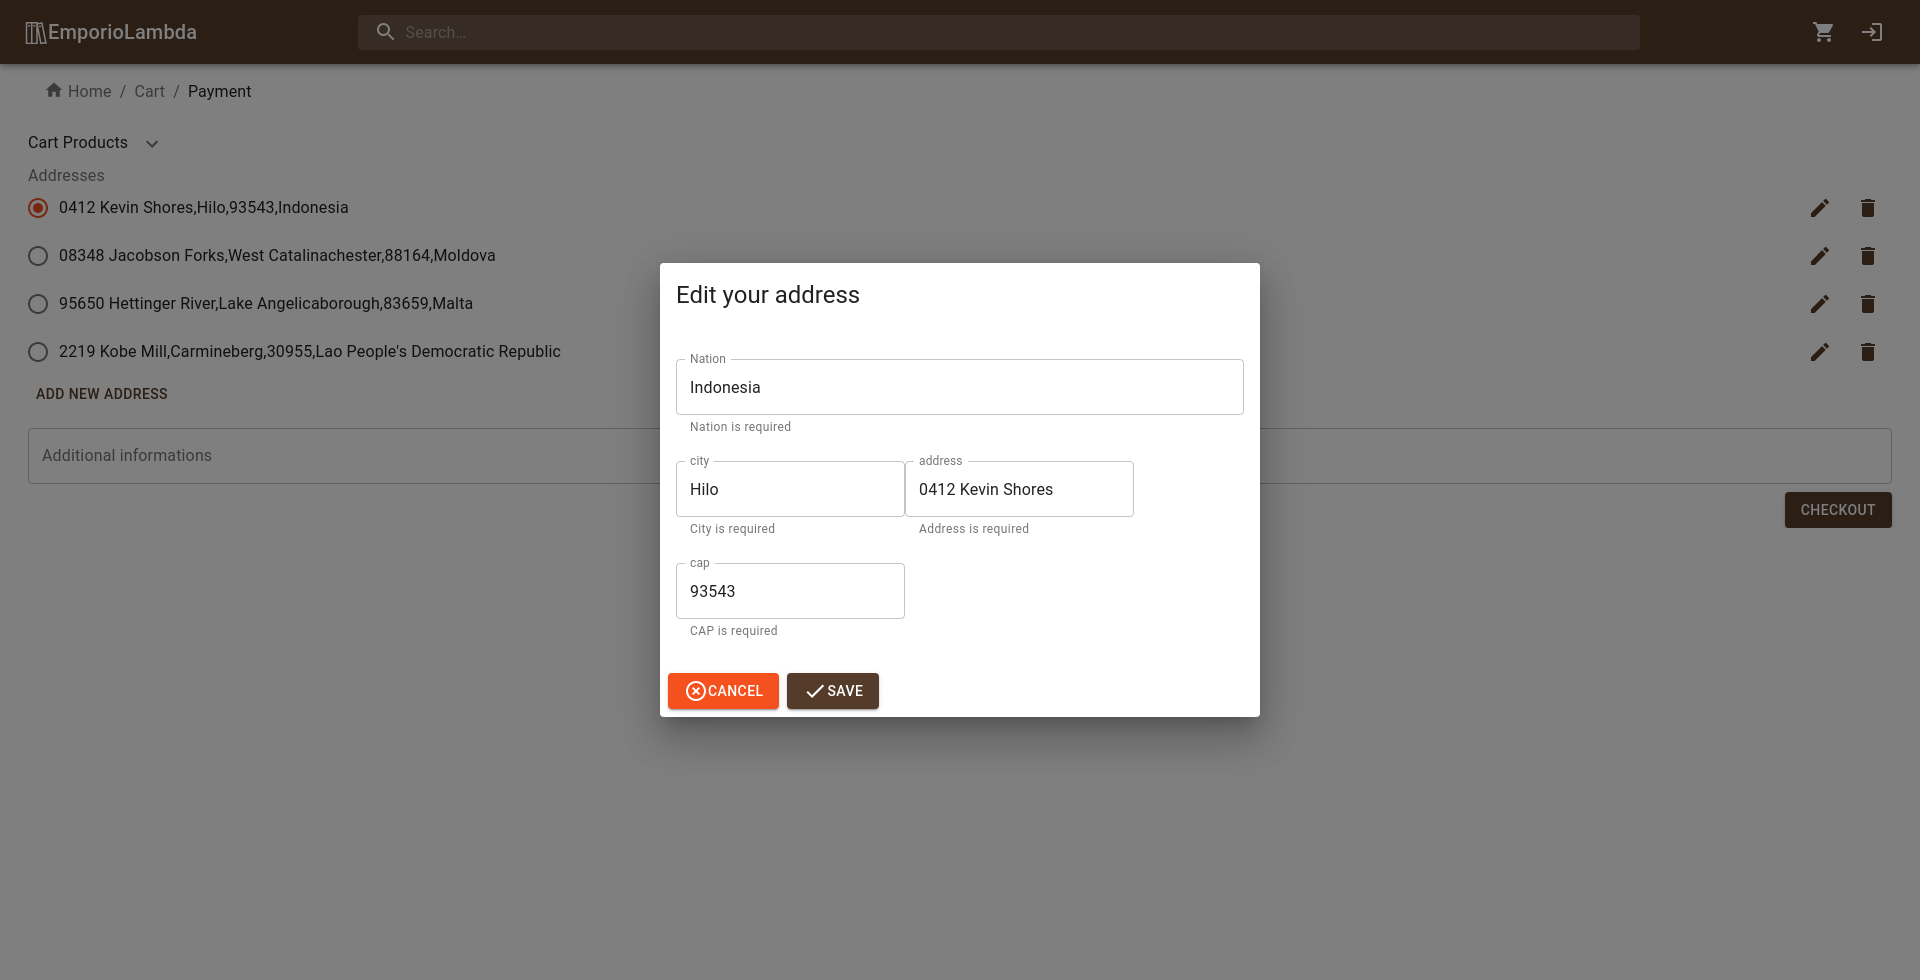
\includegraphics[scale=0.25]{Immagini/Acquirente/payment-edit-address.customer.png}
	\caption{Form per modificare l'indirizzo}
	\label{fig:CartEditAddress}
\end{figure}
\subsubsection{Procedere con il checkout}
Per procedere con il pagamento è necessario cliccare sull'apposito bottone, l'utente verrà reindirizzato alla schermata in cui inserire i dati per il pagamento e completare l'ordine.
\begin{figure}[H]
	\centering
	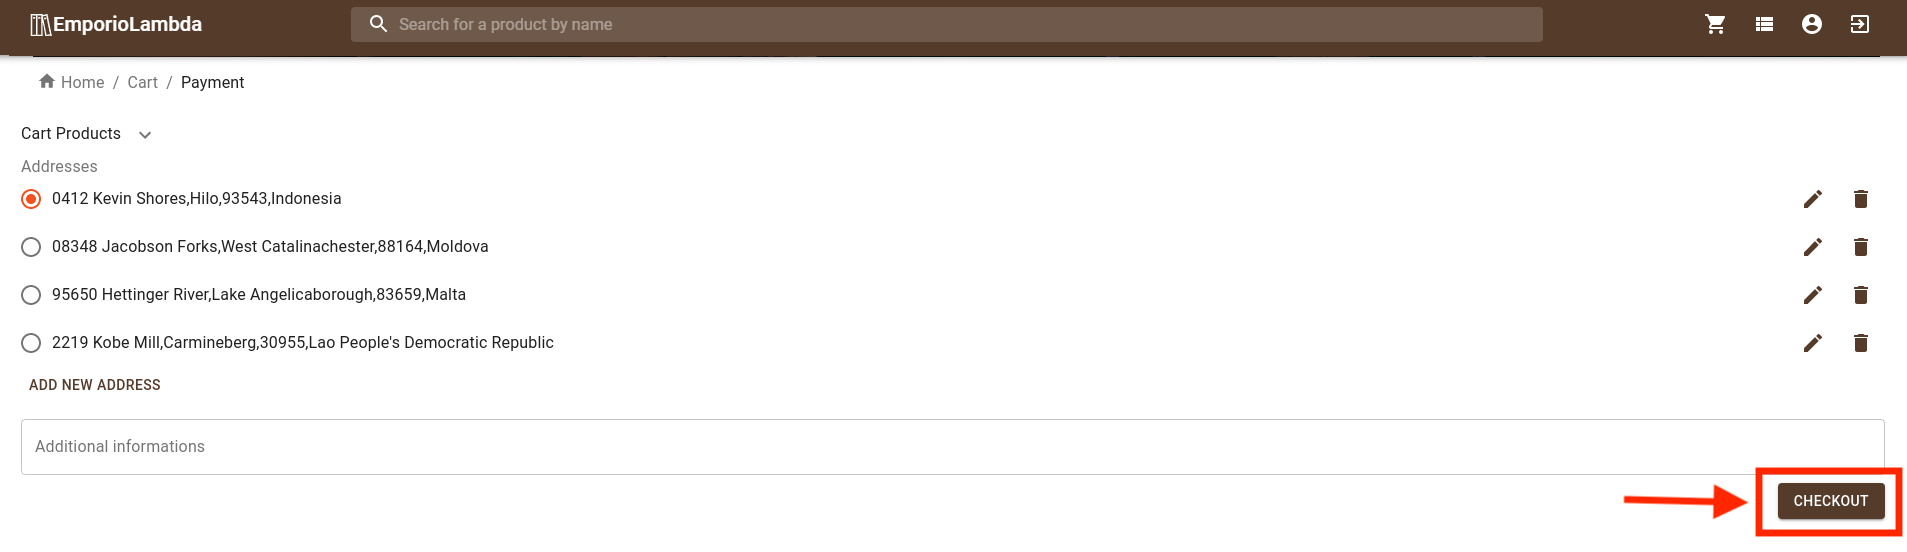
\includegraphics[scale=0.25]{Immagini/Acquirente/payment.checkout.png}
	\caption{Schermata di riepilogo prima del checkout con icona per procedere con il pagamento}
	\label{fig:CartCheckout}
\end{figure}
\newpage
\section{Venditore}\label{Venditore}
Dopo il login, l'utente autenticato come venditore visualizzerà la schermata principale della piattaforma e potrà:
\begin{enumerate}
	\item Procedere con l'aggiunta di un nuovo prodotto;
	\item Visualizzare l'elenco dei prodotti della piattaforma;
	\item Procedere con la gestione delle categorie dei prodotti;
	\item Procedere alla modifica del proprio account;
	\item Effettuare il logout;
\end{enumerate}
\begin{figure}[H]
	\centering
	
\includegraphics[scale=0.4]{Immagini/Venditore/Header.png}
	\caption{Funzioni del venditore}
	\label{fig:FunzioniVenditore}
\end{figure}
\subsection{Visualizzazione elenco prodotti}
Il venditore può visualizzare tutti i suoi prodotti presenti nella piattaforma, impostando dei filtri per gestire la ricerca. In particolare può rispetto all'acquirente visualizzare i prodotti in evidenza selezionando l'\glo{icona} apposita. 
\begin{figure}[H]
	\centering
	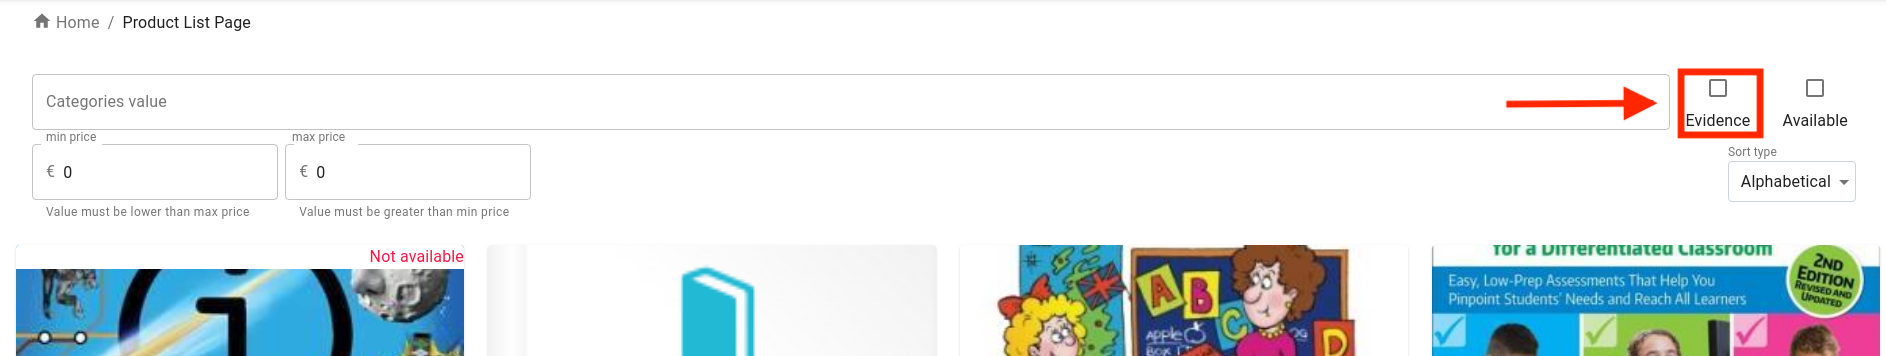
\includegraphics[scale=0.25]{Immagini/Venditore/plp.seller.png}
	\caption{Schermata prodotti con icona ricerca dei prodotti in evidenza}
	\label{fig:ProdottiEvidenza}
\end{figure}
\subsection{Gestione dei prodotti}
Il venditore può inserire, eliminare o modificare i prodotti all'interno della piattaforma.
\subsubsection{Aggiunta prodotto}
Per procedere con l'aggiunta di un nuovo prodotto, l'utente deve cliccare sull'icona (1) e verrà reindirizzato alla schermata per l'aggiunta di un prodotto.
\begin{figure}[H]
	\centering
	
\includegraphics[scale=0.4]{Immagini/Venditore/Seller Header.png}
	\caption{Barra del menù del venditore}
	\label{fig:BarraVenditore}
\end{figure}
\begin{figure}[H]
	\centering
	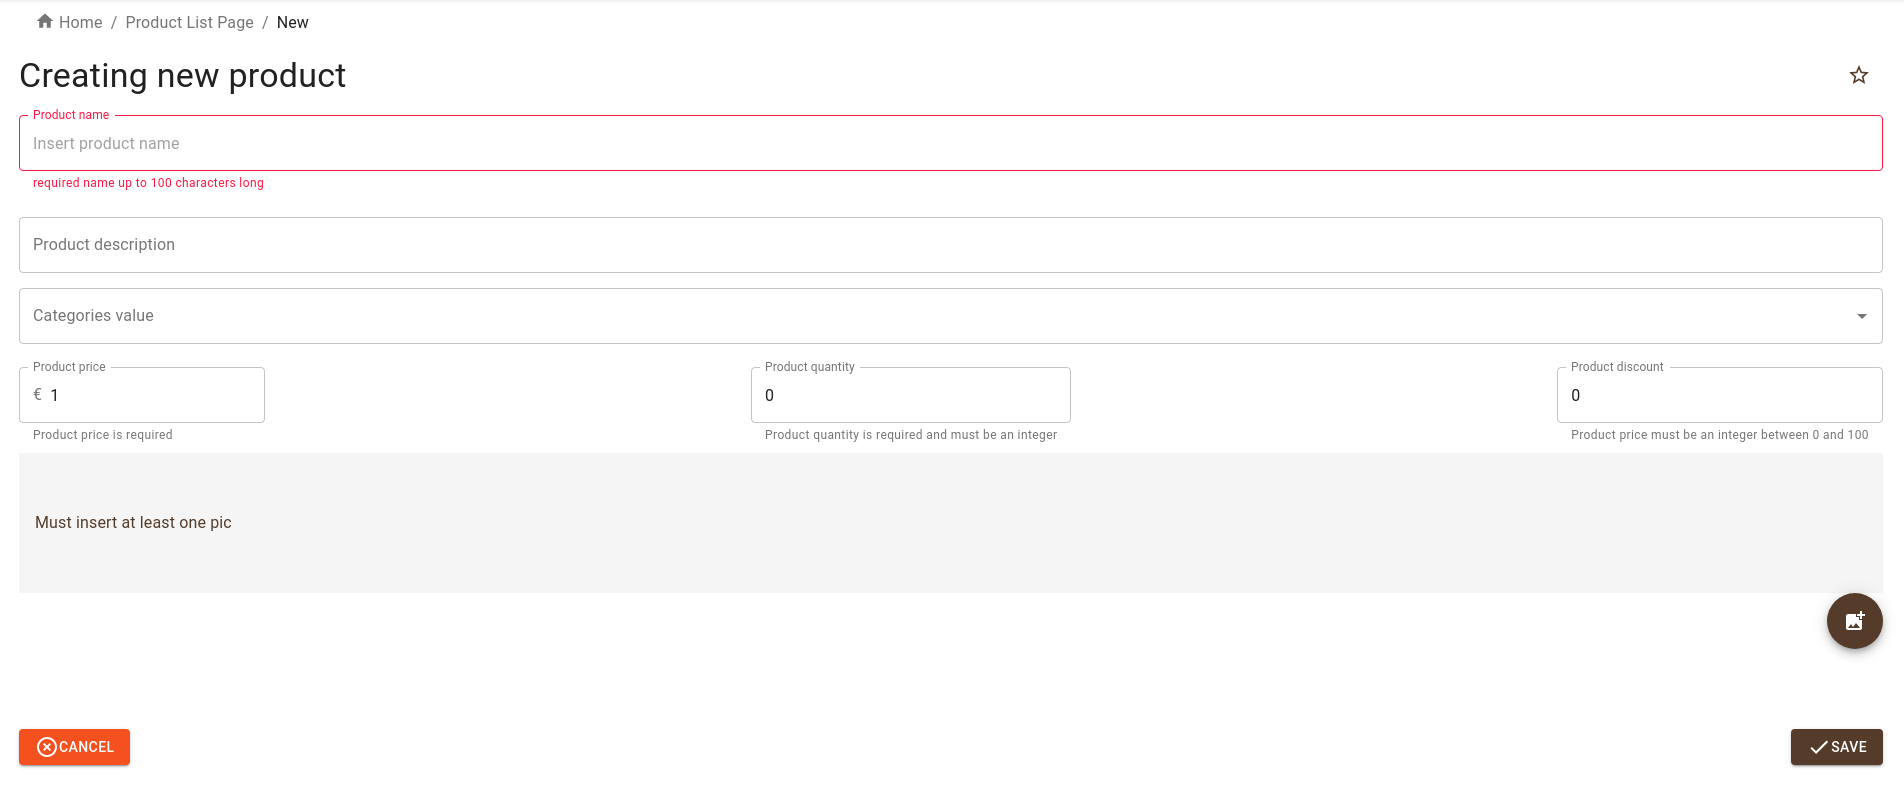
\includegraphics[scale=0.25]{Immagini/Venditore/pdp-new.seller.png}
	\caption{Aggiunta di un nuovo prodotto}
	\label{fig:AggiuntaProdotto}
\end{figure}
\subsubsection{Visualizzazione descrizione prodotto}
Il venditore può visualizzare la schermata di descrizione di un prodotto inserito e cliccando sulla icona a forma di stella posizionerà il prodotto tra quelli in evidenza.
\begin{figure}[H]
	\centering
	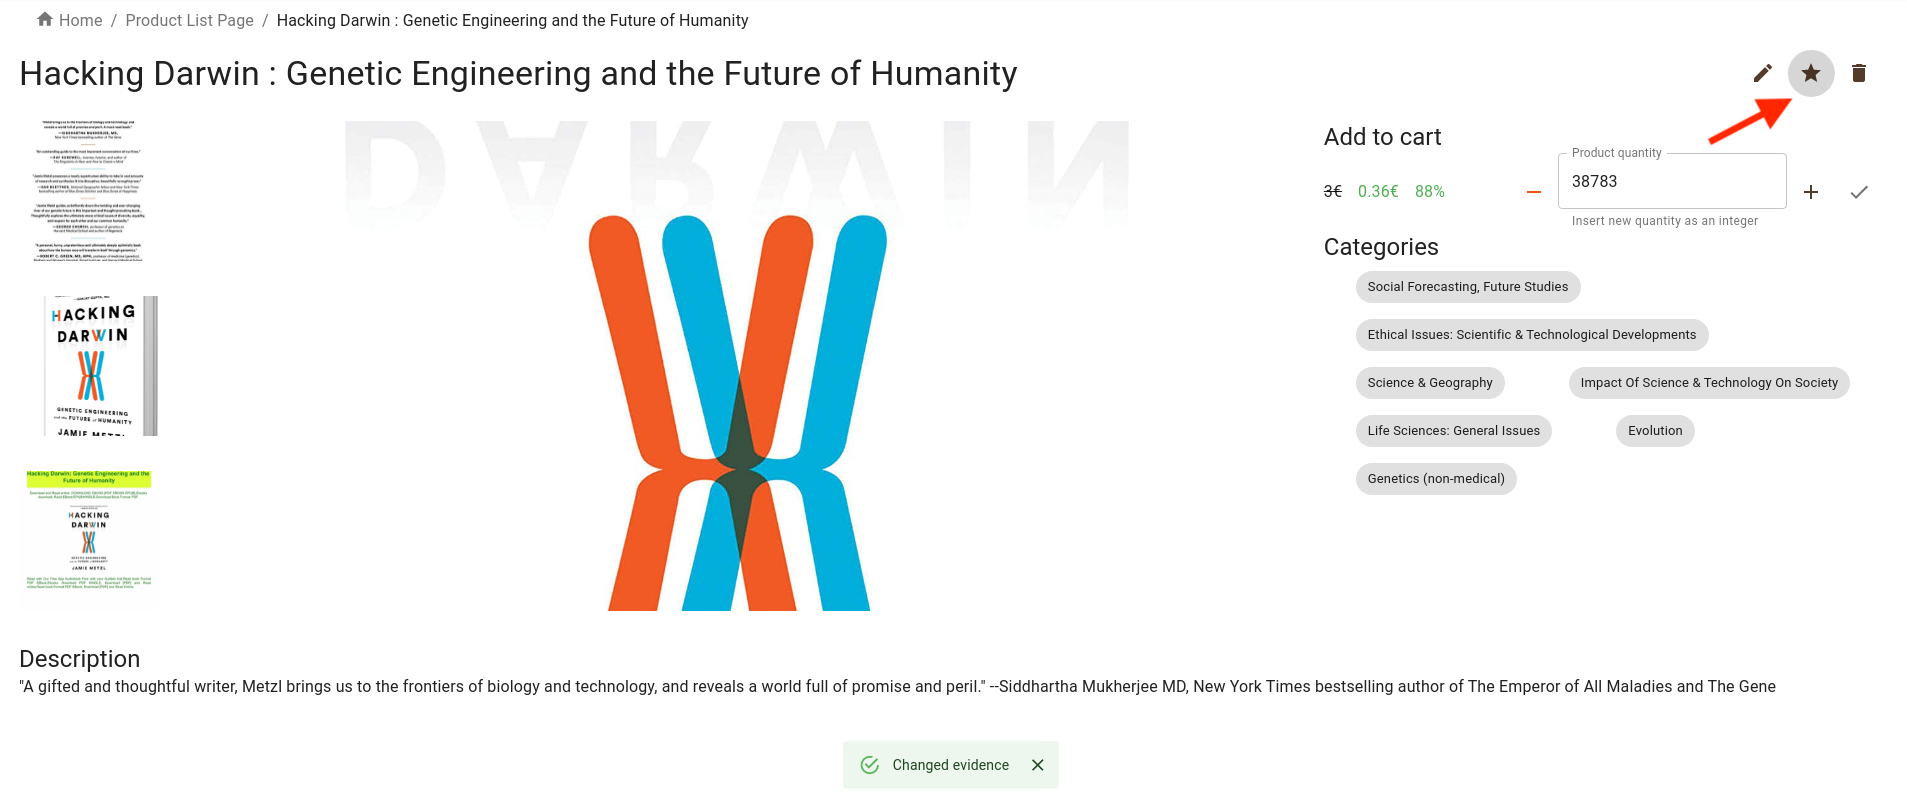
\includegraphics[scale=0.25]{Immagini/Venditore/pdp-evidence-setted.seller.png}
	\caption{Visualizzazione schermata di un prodotto in evidenza}
	\label{fig:VisualizzazioneProdotto}
\end{figure}
Per l'utente è inoltre possibile modificare la quantità disponibile del prodotto. 
\begin{figure}[H]
	\centering
	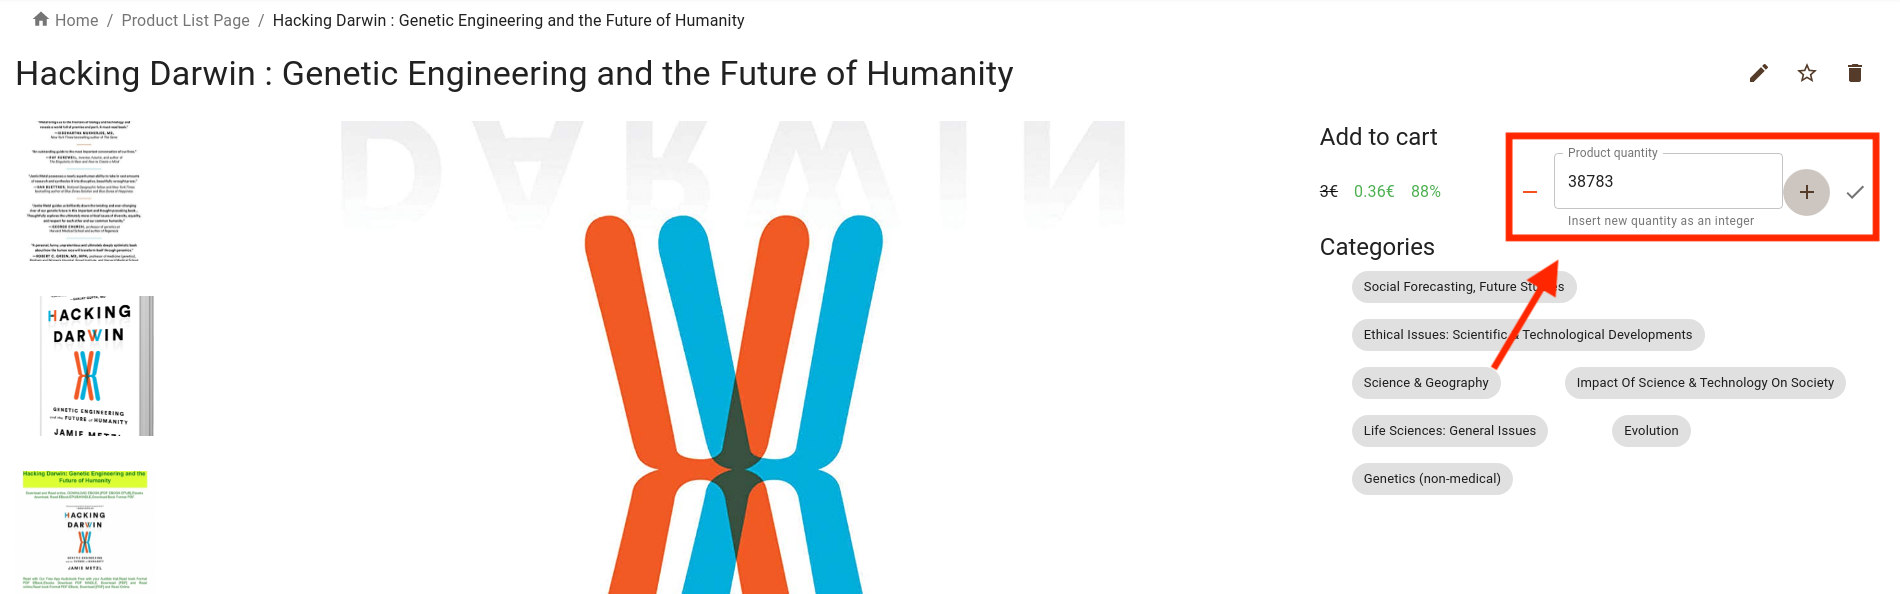
\includegraphics[scale=0.25]{Immagini/Venditore/pdp-changing-quantity.seller.png}
	\caption{Modifica quantità disponibile di un prodotto}
	\label{fig:QuantitàProdotto}
\end{figure}
\subsubsection{Eliminazione prodotto}
Per procedere con l'eliminazione di un prodotto, l'utente, dopo aver aperto la schermata di visualizzazione del prodotto che desidera eliminare, deve cliccare sull'icona del cestino e confermare la richiesta di eliminazione.
\begin{figure}[H]
	\centering
	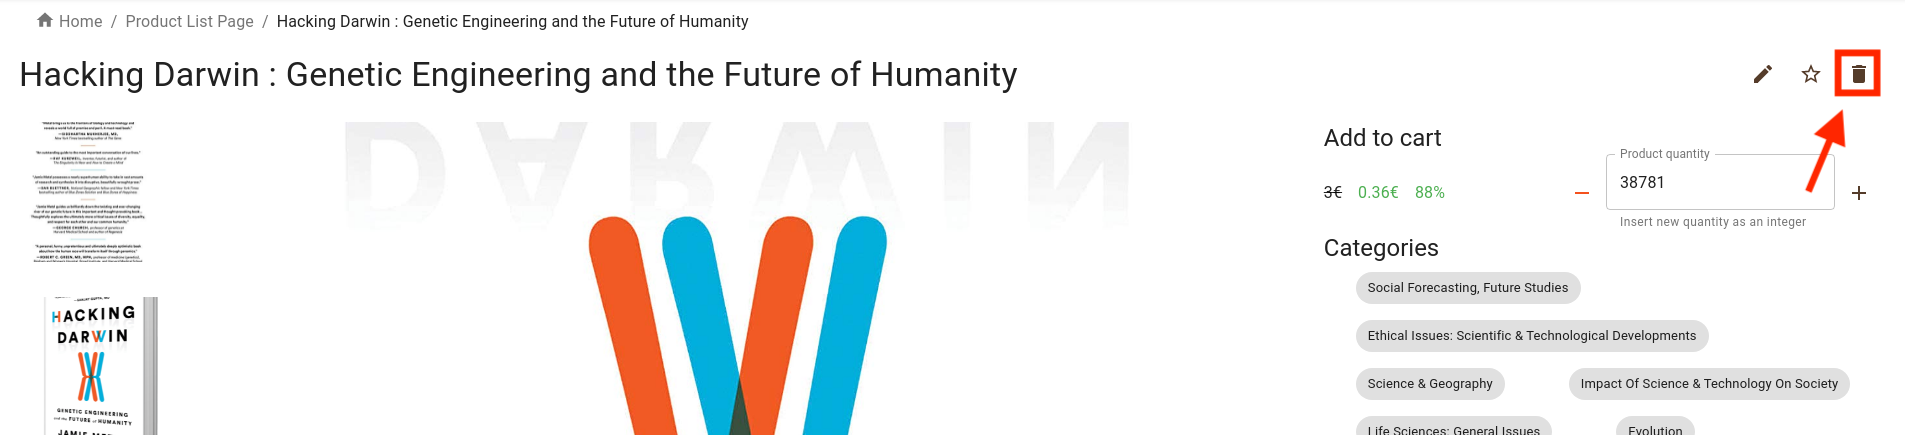
\includegraphics[scale=0.25]{Immagini/Venditore/pdp.sellerdelete.png}
	\caption{Pagina del prodotto con icona per l'eliminazione}
	\label{fig:EliminaP}
\end{figure}
\begin{figure}[H]
	\centering
	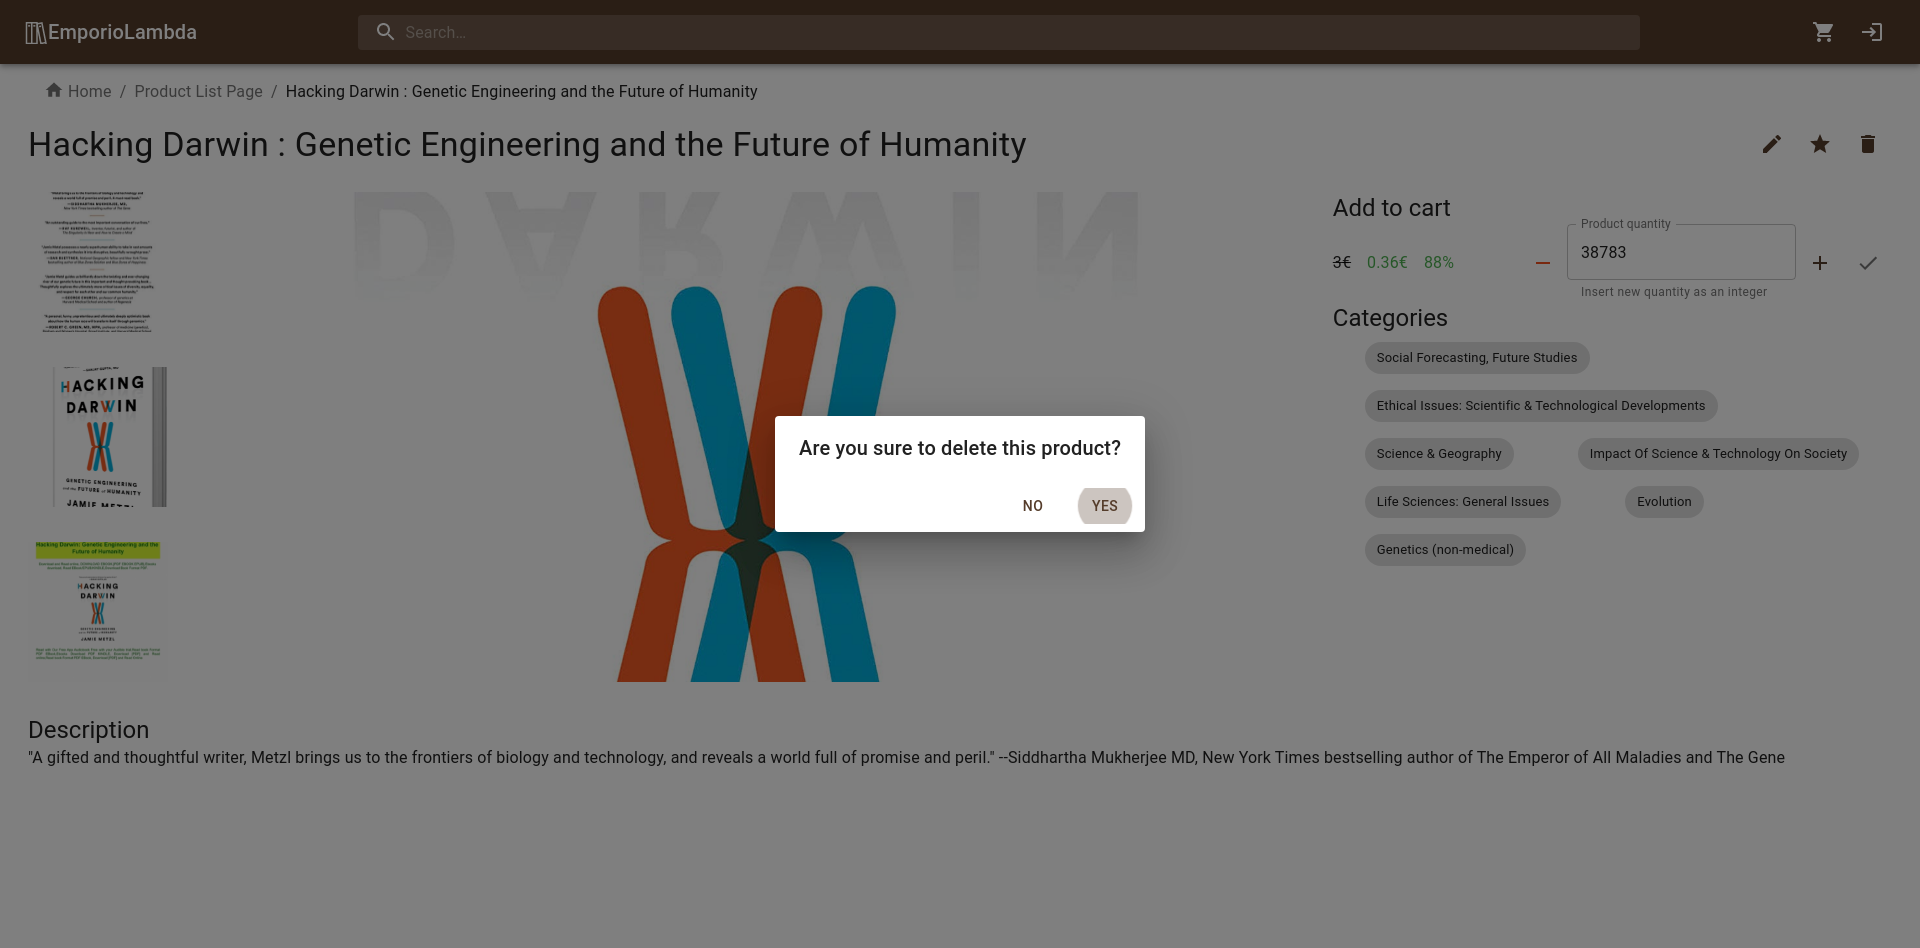
\includegraphics[scale=0.25]{Immagini/Venditore/pdp-remove.seller.png}
	\caption{Conferma eliminazione prodotto}
	\label{fig:EliminazioneProdotto}
\end{figure}
\subsubsection{Modifica prodotto}
Per procedere con la modifica di un prodotto, l'utente, dopo aver aperto la schermata di visualizzazione del prodotto che desidera eliminare, deve cliccare sull'icona del cestino e verrà reindirizzato alla pagina di modifica del prodotto.
\begin{figure}[H]
	\centering
	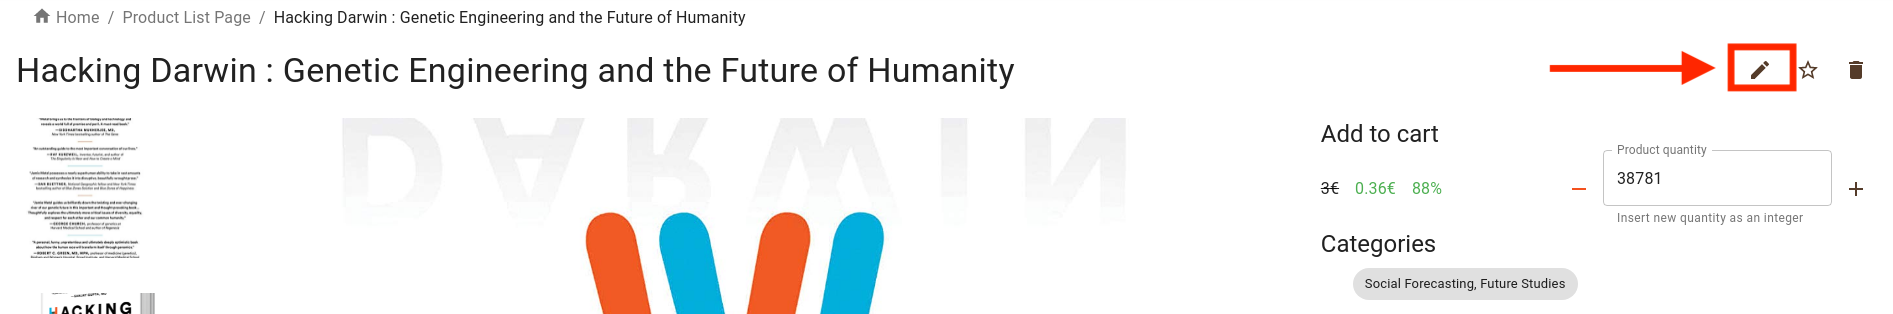
\includegraphics[scale=0.25]{Immagini/Venditore/pdp.sellermodify.png}
	\caption{Pagina del prodotto con icona per la modifica}
	\label{fig:ModificaP}
\end{figure}
\begin{figure}[H]
	\centering
	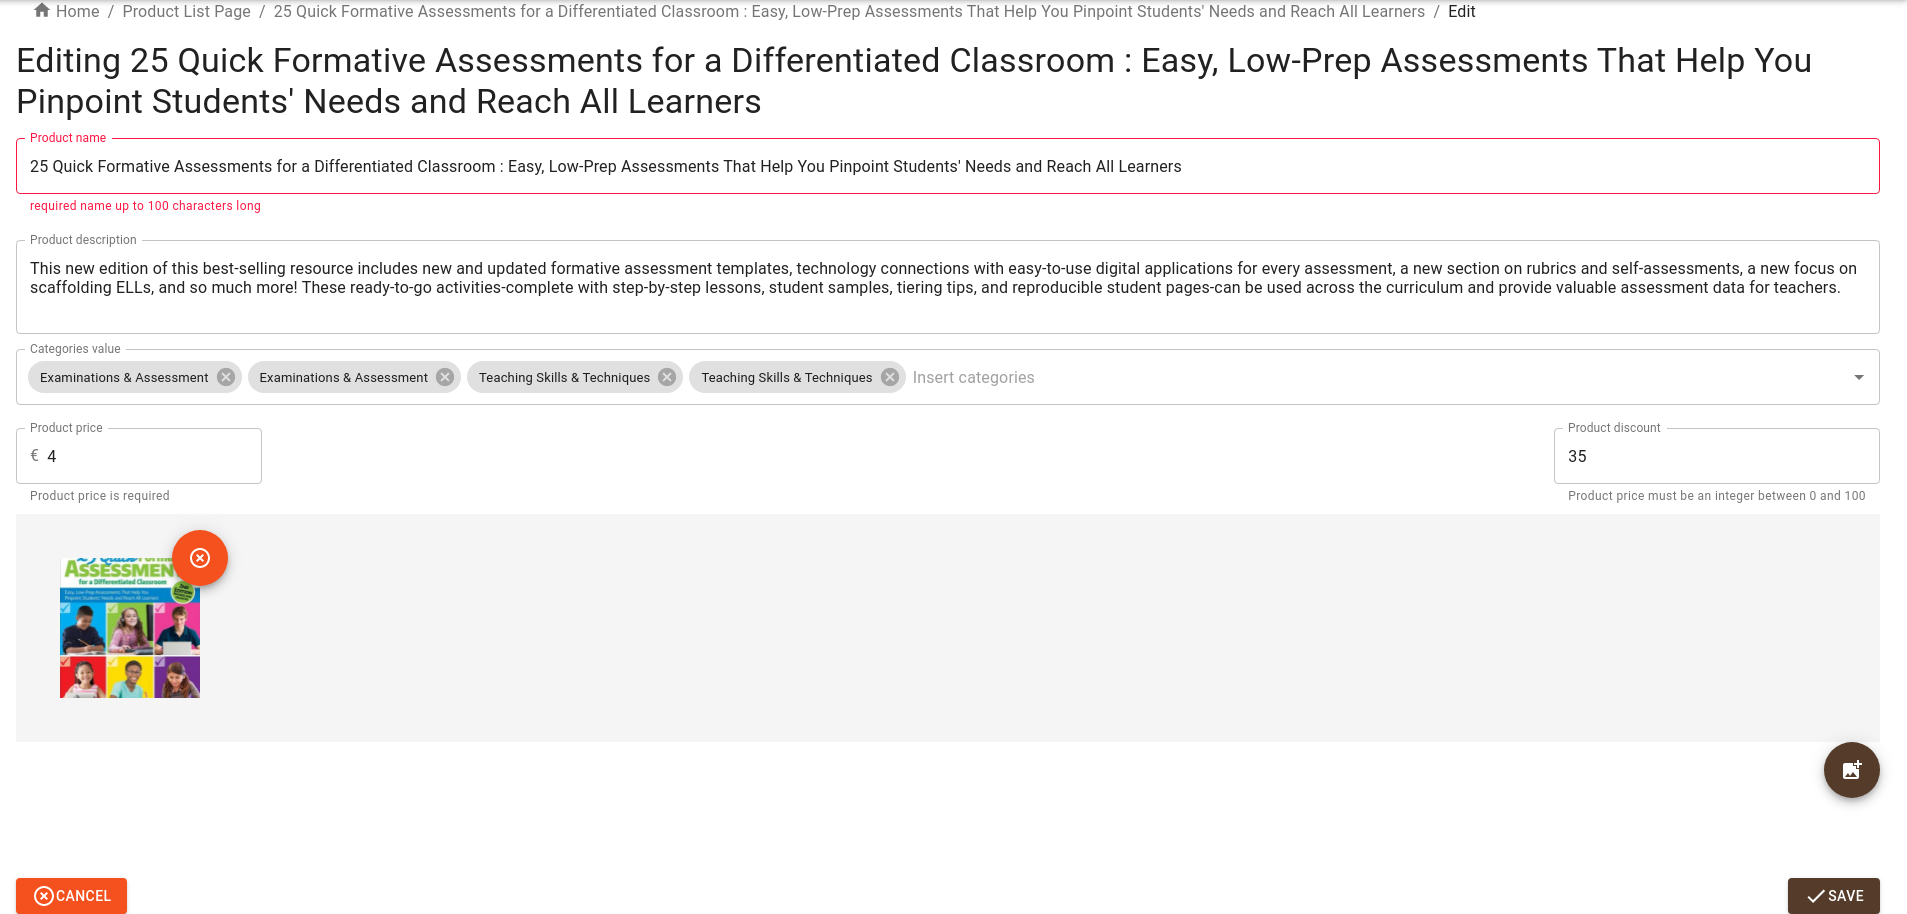
\includegraphics[scale=0.25]{Immagini/Venditore/pdp-edit.seller.png}
	\caption{Schermata di modifica prodotto}
	\label{fig:ModificaProdotto}
\end{figure}
\newpage
\section{Glossario}\label{Glossario}
\appendix
\subsection*{B}
\TermineGlossario{Browser}
\DefinizioneGlossario{
	Programma utilizzato dall'utente per navigare in Internet che inoltra la richiesta di un documento alla rete e ne consente la visualizzazione una volta arrivato.
}
\subsection*{E}
\TermineGlossario{E-commerce}
\DefinizioneGlossario{
	Piattaforma web attraverso la quale commercianti e acquirenti vengono in contatto.
}
\subsection*{F}
\TermineGlossario{Form}
\DefinizioneGlossario{
 Indica una piccola finestre in cui l'utente può inserire e inviare uno o più dati liberamente digitati dallo stesso sulla tastiera.
}
\subsection*{I}
\TermineGlossario{Icona}
\DefinizioneGlossario{
 Immagine stilizzata impiegata per rappresentare programmi, documenti, archivi di dati, singole informazioni e anche varie funzioni di un computer.
}

\end{document}